\documentclass[graybox]{svmult}

\usepackage{type1cm}         % activate if the above 3 fonts are not available on your system
\usepackage{makeidx}         % allows index generation
\usepackage{graphicx}        % standard LaTeX graphics tool when including figure files
\usepackage{multicol}        % used for the two-column index
\usepackage[bottom]{footmisc}% places footnotes at page bottom
\usepackage{newtxtext}       %
\usepackage{newtxmath}       % selects Times Roman as basic font

\makeindex             % used for the subject index please use the style svind.ist with your makeindex program



\begin{document}

\title*{Modeling Fires Using Computational Fluid Dynamics (CFD)}

\author{Kevin McGrattan and Bart Merci}

\institute{Kevin McGrattan is a mathematician in the Engineering Laboratory at the National Institute of Standards and Technology in Gaithersburg, Maryland. He is a principal developer of the Fire Dynamics Simulator (FDS). \\[0.1in]
           Bart Merci is full professor at Ghent University, Belgium. He is the head of the research unit Combustion, Fire and Fire Safety and is an expert in CFD for fire flows.}

\maketitle


\section{Introduction}

It was in the early 1920s that Lewis Richardson first demonstrated the feasibility of solving, using numerical methods, the governing equations of fluid flow~\cite{Richardson}  for the purpose of weather prediction. It was not for another 50 years that what is now known as computational fluid dynamics (CFD) emerged as a general analysis tool for the full breadth of fluid flow problems including those associated with fire.

In contrast to zone models, the techniques of CFD evolved outside the fire community and were subsequently imported into it. The same basic CFD technology is being developed, applied, verified, and validated for a wide range of applications. Problems and successes demonstrated elsewhere can often be exploited in the fire context, although there are many issues that are unique to fire that can only be the responsibility of the fire community. The same tools that are used to study, for example, heat transfer in an internal combustion engine can also be used to evaluate indoor air movement, early detection of smoke, and the dispersion of combustion products within the atmospheric boundary layer.

CFD provides the potential to study these complicated problems that are only partially amenable to reduced-scale physical modeling because of the large number of non-dimensional groups that need to be preserved to simulate full-scale behavior. Furthermore, CFD has emerged as an important tool because the assumptions employed in zone models limit their range of application to relatively simple fire scenarios that can be described in terms of a small number of idealized components ({\em e.g.}, unperturbed fire plume, unconfined ceiling jet, uniform hot gas layer).

The starting point for CFD models is the set of partial differential equations that assert conservation of mass, momentum, and energy within the fire and throughout the space surrounding it. These equations are solved numerically to yield time-varying predictions of temperature,  gas  velocity,  gas species concentrations, and so forth, on a three dimensional mesh of control volumes that spans the geometry being modeled. Unlike two zone models, CFD models enforce the conservation laws in each of the thousands or millions of relatively small control volumes. However, the exact solution of the governing equations, resolving fully the length and time scales that occur in the turbulent flows associated with fire, is still beyond the capabilities of even the largest computers currently available. To capture the details of the chemical processes of a fire would require spatial resolution of less than 1 millimeter. As a consequence, it is necessary to modify the governing equations to model the unresolvable turbulence. Two main approaches are currently employed in CFD simulations of fire: large eddy simulation (LES) and Reynolds-averaged Navier-Stokes (RANS) equations, which are described later in this chapter.

In addition to the uncertainties associated with the modeling of turbulent flow, others are introduced by the description of combustion chemistry; radiation; and mass, momentum, and heat transfer at solid boundaries. Further complexity is introduced in the numerical solution of the equation set in which the choice of numerical schemes and the resolution of the numerical mesh strongly influences the quality of the CFD solution. An appreciation of all these issues is important in the successful exploitation of CFD to solve fire problems.
It should be recognized that this topic is rapidly evolving and that this chapter can only represent a ``snapshot'' in time. Whereas a thousand mesh points constituted a detailed CFD solution in the early 1980s, simulations using millions of mesh points are now routine. This number can be expected to increase further, especially as parallel processing becomes more widespread. However, although the modeling of smoke transport may be considered reasonably mature, there remains considerable research and development still to be done with some of the more complex issues related to the underlying combustion and fire science ({\em e.g.}, flame spread, oxygen vitiation, soot formation, and water suppression). Here the challenges remain considerable and will not be satisfactorily solved for some time yet.

This chapter does not provide a comprehensive description of CFD. There are already numerous introductory textbooks on the subject~\cite{Anderson, Ferziger, Patankar, Peyret, Versteeg}. Depending on the background of the author(s), these books tend to emphasize techniques developed for particular fields of science and engineering, such as aerospace, meteorology, or combustion. Discussion of issues related to the modeling of fire can be found in review articles by Cox~\cite{Cox:1995,Cox:1998}  and Novozhilov~\cite{Novozhilov}. Finally, a comprehensive description of the specific algorithms used by a particular CFD model can only be found within the manuals that accompany the software. A recent review by Olenick and Carpenter~\cite{Olenick} lists about a dozen CFD models developed specifically for fire. Some of these models were developed for specific fire scenarios or phenomena. Others were developed to handle a variety of fire scenarios, including JASMINE from the Fire Research Station (U.K.), the Fire Dynamics Simulator (FDS) from NIST (U.S.) and VTT (Finland), SMARTFIRE from the University of Greenwich (U.K.), and SOFIE, the product of a European consortium. A more recent development is the FireFOAM model from FM Global, which is based on the open source CFD code OpenFOAM. There are also general-purpose CFD models that have been used for fire simulations. These computer programs contain tens to hundreds of thousands of lines of instructions, along with manuals that contain hundreds of pages of documentation of the development, algorithms, and validation of the models.

This chapter provides an introduction to the theory and practice of computational fluid dynamics as applied to the study of fire. Although the mathematical framework for the subject is more than 100 years old, it is only in the past 30 years that computers have become fast enough to make the models practical.


\section{Governing Equations}

This section presents the conservation equations of mass, momentum, and energy that are typically applied in CFD models of fire. The derivation of these equations can be found in any textbook on the subject and are discussed only briefly here. Instead, the focus shall be on assumptions and approximations that are typically applied to fire modeling.

\subsection{Coordinate System}

In its most basic form, a CFD model is essentially a discretized form of the mass, momentum, and energy conservation equations. The term {\em discretized} means that the continuous equations are approximated over relatively small control volumes, or {\em grid cells}. The conservation equations are derived under the assumption that mass, momentum, and energy are conserved as the fluid flows in and out of the grid cells. It is convenient in fire to think in terms of small, rectangular boxes because the overall computational domain is often a collection of rectangular rooms, hallways, stairwells, etc. It is also convenient to adopt a Cartesian coordinate system such that any point in three space is defined by the spatial coordinates $\mathbf{x}=(x,y,z)$. The coordinate $z$ is usually applied to the vertical direction, and the coordinate system conforms to the right-hand rule.

CFD applied to other fields of engineering may adopt other coordinate systems that are more convenient. For example, global weather modeling might employ a spherical coordinate system. Aerospace applications might employ a cylindrical coordinate system with body-fitted grid cells surrounding the object of interest.


\subsection{Physical Quantities of Interest}

The solution of the discretized conservation equations yield fundamental properties of the fluid in each grid cell at a set of discrete time steps. CFD fire models typically treat the fluid as a mixture of ideal gas species. The {\em mass fraction} of each species, $Y_\alpha$, is the ratio of the mass of that species to the total mass of the mixture. These are non-dimensional quantities, and they sum to 1, $\sum_\alpha Y_\alpha = 1$. Likewise, the density of the gas mixture can be decomposed into components, $\rho = \sum_\alpha \rho Y_\alpha$. Thus, knowing the mass fractions of all the gas species is equivalent to knowing the density. The unit for density is typically kg/m$^3$.

The velocity of the gas mixture is expressed by the vector $\mathbf{u}=(u,v,w)$. Each component of velocity is a function of space and time. The unit for velocity is typically m/s.

The pressure, $p$, is typically decomposed into components:
\begin{equation}
   p(\mathbf{x},t) = p_\infty - \rho_0(z) g z + \tilde{p}(\mathbf{x},t)
\end{equation}
where $p_\infty$ is the pressure at ground level or other fixed reference point, $\rho_0$ is the initial or ambient background density field which is only a function of the vertical coordinate $z$, and $\tilde{p}$ is the perturbation pressure that drives the flow. The unit for pressure is typically the Pascal, Pa.

The temperature of the gas mixture is typically not solved for directly, but rather the {\em specific enthalpy}:
\begin{equation}
  h_{\rm s} = \sum_\alpha h_{{\rm s},\alpha}(T) \, Y_\alpha \quad ; \quad h_{{\rm s},\alpha}(T) = \int_{T_{\rm ref}}^T c_{p,\alpha}(T') \, \mbox{d}T'
\end{equation}
The values of the temperature-dependent, specific heats, $c_{p,\alpha}(T)$, are typically tabulated in reference handbooks. The unit for specific enthalpy and specific heat are typically J/kg and J/(kg$\cdot$K), respectively.



\subsection{Conservation of mass}

The conservation equations are typically derived by considering a fixed, closed volume, $\Omega$, bounded by the surface, $\partial \Omega$. Conservation of mass asserts that the rate of change of the mass of each gas species $\alpha$ within the volume is equal to the amount of species $\alpha$ (1) flowing into the volume, (2) diffusing into the volume, or (3) being generated via chemical reactions:
\begin{equation}
   \frac{ \partial }{\partial t} \int_\Omega  (\rho Y_\alpha) \, {\rm d}V = -\int_{\partial \Omega} (\rho Y_\alpha \mathbf{u}) \cdot {\rm d}{\mathbf S} + \int_{\partial \Omega} (\rho D_\alpha \nabla Y_\alpha) \cdot {\rm d}\mathbf{S} + \int_\Omega \dot{m}_\alpha''' \, {\rm d}V
   \label{eq:spec_con_vol}
\end{equation}
This equation can be rewritten (using Green's Theorem) in an alternative form favored by modelers who employ a {\em finite-difference} as opposed to a {\em finite-volume} formulation of the governing equations:
\begin{equation}
\frac{\partial (\rho Y_\alpha)}{\partial t} + \nabla \cdot (\rho Y_\alpha \mathbf{u}) = \nabla \cdot \left( \rho D_\alpha \nabla Y_\alpha \right) + \dot{m}_\alpha'''
\label{eq:speccon}
\end{equation}
When all of the species equations are added together, the mass diffusion and production terms on the right-hand side sum to zero, yielding a conservation equation for total mass:
\begin{equation}
\frac{\partial \rho}{\partial t} + \nabla \cdot \rho \mathbf{u} = 0
\label{eq:masscon}
\end{equation}
Notice that the source and diffusion terms sum to zero:
\begin{equation}
   \sum_\alpha  \dot{m}_\alpha''' = 0 \quad ; \quad \sum_\alpha \rho D_\alpha \nabla Y_\alpha = 0
\end{equation}
Note that in CFD fire models, it is common practice to apply Ficks law:
\begin{equation}
   \mathbf{J_\alpha} = -\rho D_\alpha \nabla Y_\alpha
\end{equation}
The diffusion coefficient, $D_\alpha$, provides the relationship between the diffusion flux $\mathbf{J}_\alpha$ of species $\alpha$ and the spatial gradient of the local mass fraction, $Y_\alpha$. The minus sign expresses that the diffusion flux is always from higher concentration to lower concentration. The unit of $D_\alpha$ is typically m$^2$/s.

\subsection{Conservation of Momentum}

The conservation equation for momentum is
\begin{equation}
\frac{\partial (\rho \mathbf{u})}{\partial t} + \nabla \cdot (\rho \mathbf{u} \mathbf{u}) = -\nabla p + \nabla \cdot \mu \left( \nabla \mathbf{u} + (\nabla \mathbf{u})^T \right) +  \nabla (\lambda \nabla \cdot \mathbf{u}) + \rho \mathbf{g}
\label{eq:momcon}
\end{equation}
The momentum equation is written in compact notation here to emphasize that it is essentially Newton's Second Law of Motion, which states that the change in momentum of a small parcel of fluid is proportional to the forces applied. The forces that drive the fluid consist of the pressure gradient, $\nabla p$, friction, and buoyancy, $\rho \mathbf{g}$. A complete expansion of the various terms can be found in the Appendix.

The viscosity, $\mu$, is a function of temperature and gas composition, and is obtained via table look-up. The second coefficient of viscosity, $\lambda$, is typically assumed to be related to the viscosity, $\lambda \approx -2/3 \, \mu$. In large-scale fire modeling of turbulent fires, as opposed to small-scale modeling of laminar flames, the exact form of $\mu$ and $\lambda$ are not relevant because these terms are replaced by expressions related to the {\em turbulence model}, a topic discussed in Section~\ref{section:turbulence}.

\subsection{Conservation of Energy}

The conservation equation for energy is
\begin{equation}
\frac{\partial (\rho h_{\rm s})}{\partial t} + \nabla \cdot (\rho h_{\rm s} \mathbf{u}) = \frac{Dp}{Dt} + \dot{q}''' - \nabla \cdot \mathbf{q}'' + \epsilon
\label{eq:encon}
\end{equation}
As in the mass conservation equation, the sensible enthalpy, $h_{\rm s}$, at a given point changes according to the net energy flux across the boundary of a small control volume surrounding the point. Now, however, there are additional source terms on the right-hand side of the equation related to the pressure, combustion heat release rate, radiation and conduction, and kinetic energy dissipation, respectively. For fire applications, the contributions from the pressure term and the dissipation term are negligible, except in situations where the compartment of interest is sealed and the pressure rises substantially.

The heat release rate per unit volume, $\dot{q}'''=-\sum_\alpha \dot{m}_\alpha''' h_{{\rm f},\alpha}$, where $h_{{\rm f},\alpha}$ is the heat of formation of gas species $\alpha$. The total heat release rate of the fire, $\dot{Q}=\int \dot{q}'''  {\rm d}V$, where $V$ is the volume of the entire domain.

The term $\mathbf{q}''$ represents the conductive, diffusive, and radiative heat fluxes:
\begin{equation}
   \mathbf{q}'' = -k \nabla T - \sum_\alpha h_{\rm s,\alpha}  \rho  D_\alpha \nabla Y_\alpha + \mathbf{q}_{\rm r}''  \label{bqdot_def}
\end{equation}
where $k$ is the thermal conductivity and $D_\alpha$ is the diffusivity of species $\alpha$.

\subsection{Equation of State}

The conservation equations described above provide the density of each gas species, three components of velocity, and the sensible enthalpy. However, to close the system, an {\em equation of state} is needed to relate the pressure, $p$, to the other thermodynamic variables. For most fire applications, it is sufficient to assume a {\em perfect gas}:
\begin{equation}
p = \frac{\rho {\cal R} T}{\overline{W}} \quad ; \quad \overline{W} = \frac{1}{\sum_\alpha (Y_\alpha / W_\alpha)}
\label{eq:pgas}
\end{equation}
where ${\cal R}$ is the universal gas constant and $\overline{W}$ is the average molecular weight of the gas mixture.


\subsection{Additional Assumptions}

The foregoing equations form the basis for a wide variety of engineering applications but not without the further application of simplifying assumptions unique to each field. The only assumptions made thus far are that the fluid is a perfect gas and that the viscous stress is linearly dependent on the strain. A further approximation can be made here, exploiting the fact that fire-driven flows are substantially slower than the speed of sound. By assuming that the pressure is constant (or at most a time-varying average) in the equation of state and the energy equation, the number of unknowns is reduced from six to five, as temperature can now be found from the density. More importantly, there is no longer a need to account for pressure fluctuations that propagate at the speed of sound, a fact that makes the numerical solution of the equations more tractable because the time step size is limited only by the flow speed, not the sound speed~\cite{Rehm}.

In the sections to follow, additional assumptions will be imposed on the governing equations to apply them to fire and other low-speed thermal processes. Most important is the treatment of the diffusive and source terms that distinguishes one type of CFD model from another.


\section{Turbulence Modeling}
\label{section:turbulence}


\subsection{Reynolds Averaging}

In a turbulent flow, flow quantities, like a velocity component or the temperature, at a particular location exhibit fluctuating time histories that cannot be completely resolved by the discrete time step used in the solution of the governing equations. Consider a time period $\Delta t$ that is relatively long compared to the largest turbulent time scales, but sufficiently short compared to fluctuations in the mean flow. The mean value of the quantity, in this case the $x$ component of velocity, can be defined:
\begin{equation}
   \overline{u}(\mathbf{x},t) = \frac{1}{\Delta t} \int_{t-\Delta t}^t  u(\mathbf{x},t') \, {\rm d}t'
\end{equation}
The instantaneous value, $u$, can be expressed as the sum of the {\em Reynolds-averaged} value, $\bar{u}$, and the relatively high frequency, randomly fluctuating component, $u'$:
\begin{equation}
   u(\mathbf{x},t) = \overline{u}(\mathbf{x},t) + u'(\mathbf{x},t)
\end{equation}
Noting that 
\begin{equation}
\overline{u'}=0 \quad ; \quad \overline{\overline{u}} = \overline{u} \quad ; \quad \overline{uv} = \overline{ (\overline{u}+u')(\overline{v}+v')} = \bar{u}\bar{v} + \overline{u'v'}
\end{equation}
this averaging technique can be applied to the conservation equations, and a slightly modified set of equations is obtained for the Reynolds-averaged quantities. They are very similar to the original equations, but some additional terms appear---Reynolds stresses in the momentum equations and turbulent heat fluxes in the energy equation. 

The derivation of the Reynolds-averaged Navier-Stokes equation is included in any textbook on CFD. As a simple example, consider a vertical, flat wall with a steady stream of constant-temperature air flowing horizontally, as shown in Fig.~\ref{eddy_diagram}. The Reynolds-averaged mass and momentum equations can be greatly simplified because the time derivatives of the mean flow drop out, the density, $\rho$, is constant, and force terms like the pressure gradient and gravity drop out as well, leaving:
\begin{equation}
   \frac{\partial \bar{u}}{\partial x} + \frac{\partial \bar{v}}{\partial y} = 0 \quad ; \quad
   \bar{u} \frac{\partial \bar{u}}{\partial x} + \bar{v} \frac{\partial \bar{u}}{\partial y} = \frac{\partial}{\partial y} \left( \frac{\mu}{\rho} \frac{\partial \bar{u}}{\partial y} \right) -  \frac{\partial}{\partial y} \left( \overline{u'v'} \right) \label{bleq}
\end{equation}
These equations for the Reynolds-averaged velocity components are identical to the original equations except for the second term of the momentum equation. This term is non-zero only if $u'$ and $v'$ are statistically correlated. This is the case, as explained with the schematic in Fig.~\ref{eddy_diagram}. In turbulent flows such as this, eddies form due to wall fraction. Typically these eddies cannot be {\em resolved}; that is, they are too small relative to the underlying numerical grid, as highlighted in Fig.~\ref{vector_plot}. Looking at the simplified eddy in Fig.~\ref{eddy_diagram}, its instantaneous motion on its left side is in the negative $y$ direction ($v'<0$). This motion draws air with a relatively high mean velocity in the $x$ direction into a region with a lower mean velocity; thus, $u' > 0$. From a statistical point of view, the velocity fluctuations in both directions are correlated, $\overline{u'v'} < 0$. At the right side of the eddy, the instantaneous motion is upward ($v' > 0$) and air with a relatively low mean velocity is brought into a region with a relatively high mean velocity, causing $u' < 0$. Thus, again $\overline{u'v'}<0$.

\begin{figure}[ht]
\setlength{\unitlength}{1cm}
\begin{picture}(10,5)(-1,-1)
\put(4,1.5){\circle{0.5}}
\put(4.25,1.5){\vector(0, 1){0.5}}
\put(3.75,1.5){\vector(0,-1){0.5}}
\put(0,0){\vector(1,0){3}}
\put(0,0){\vector(0,1){3}}
\put(0,0.5){\vector(1,0){0.5}}
\put(0,1.0){\vector(1,0){1.0}}
\put(0,1.5){\vector(1,0){1.5}}
\put(0,2.0){\vector(1,0){2.0}}
\put(0,2.5){\vector(1,0){2.5}}
\put(-0.2,3.0){$y$}
\put(3.0,-0.2){$x$}
\put(0.9,2.75){$\bar{u}(x,y)$}
\put(2.75,1.0){$v'<0$}
\put(4.40,1.75){$v'>0$}
\end{picture}
\caption{Schematic diagram of a small eddy in the presence of a boundary layer flow.}
\label{eddy_diagram}
\end{figure}


\begin{figure}[p]
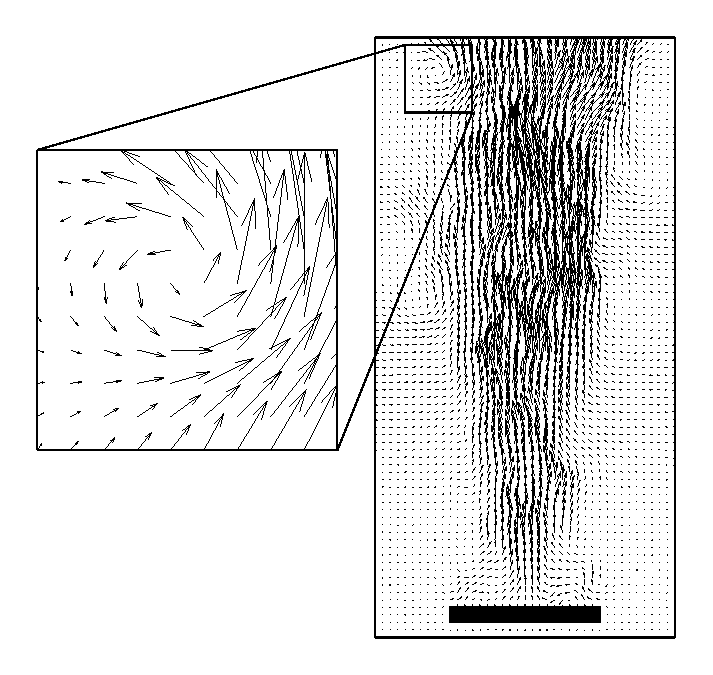
\includegraphics[width=\textwidth]{Fig_plume_vectors}
\caption{What is meant by ``resolvable.'' At right is an instantaneous map of the flow vectors for an LES simulation of a helium plume. the inset shows the smallest ``eddy'' that can be supported by the numerical grid, the spacing of which is indicated by the distance between the arrows.}
\label{vector_plot}
\end{figure}


This type of argument led to the following ``eddy viscosity'' modeling concept, introduced by Boussinesq:
\begin{equation}
-\overline{u'v'} = \frac{\mu_{\rm t}}{\rho} \frac{\partial \bar{u}}{\partial y}
\end{equation}
In other words, a ``turbulent'' or ``eddy'' viscosity is simply added to the molecular viscosity in Eq.~(\ref{bleq}). The form of the eddy viscosity is the subject of the next section.


\subsection{Turbulence Modeling}

The purpose of the eddy viscosity is to model the transfer of energy at length and time scales that are unresolved by the mean flow variables. The largest turbulence scales are called the {\em integral} scales. The smallest scales are called the {\em Kolmogorov} scales. A detailed discussion of the spectrum is considered beyond the scope of this section, but suffice it to say that most of the turbulent kinetic energy is in the integral scales, while turbulence is dissipated at the Kolmogorov scales where viscous damping converts the turbulent kinetic energy into heat. The notion of energy cascade, introduced by Richardson, is worth mentioning:
\begin{itemize}
\item Energy is taken from the mean flow and transferred to kinetic energy of turbulent eddies; this occurs around the integral scales; 
\item The turbulent eddies break up, transferring their energy to the eddies of smaller scale; a relatively small amount of energy is dissipated at this stage;
\item The break-up process, or {\em cascade}, of eddies continues until the eddies become so small that they cannot survive the damping action of viscosity;
\item The dissipation takes place at the smallest turbulence scales.
\end{itemize}
Whereas the dissipation takes place at the smallest scales, the dissipation rate is determined by the production rate of turbulence from the mean flow in the energy containing range. This phenomenology is reflected in the choice of turbulence model. One extreme approach is not to model turbulence at all, but rather to resolve completely all turbulent motion down to the smallest scales. However, these small scales are typically on the order of 1~mm or less, requiring an excessive amount of computing resources. Making matters worse, most of the computer time and memory is devoted to simulating the smallest scales~\cite{Pope:2000}, whereas the primary interest is typically in the large scale flow phenomena.

The other extreme in turbulence modeling is known as RANS (Reynolds-Averaged Navier-Stokes). In this approach, Reynolds averaging is applied and all turbulent motion, i.e. the entire turbulent spectrum is modeled. Only the mean flow is resolved. For example, a fire plume simulated with a RANS model does not exhibit the characteristic pulsations and large eddy formation as shown in Fig.~\ref{vector_plot}. Rather, a steady upward flow field results, and the action of the pulsation and large eddy formation is modeled with relatively large diffusive terms in the momentum and energy equations. The advantages of the RANS approach are that the computational mesh only needs to be fine enough to resolve the mean flows, and the time step (in transient calculations) can be chosen on the basis of mean flow phenomena. There are major disadvantages, however. First, all turbulence is modeled. Knowing that the largest turbulent scales are configuration dependent, it cannot be expected that a single RANS model can deal with arbitrary configurations in a reliable manner. Second, in fire related flows large scale flow unsteadiness often plays an important role; for example, in the entrainment process of a fire plume. Such unsteadiness is not captured in (unsteady) RANS and must be modeled. Again, being configuration dependent, RANS models cannot be expected to be as accurate as approaches where this unsteadiness is resolved.

This explains the popularity of the LES (Large-Eddy Simulations) technique in CFD for fire related flows. In this technique, the large scale eddies are resolved and only the effect of the small scale eddies is modeled. This technique offers the advantage of resolving the large-scale flow unsteadiness (and buoyancy effects). Also, the unacceptable fineness of the computational mesh as required in DNS is avoided. Yet, there is a very important caveat. Indeed, in order to guarantee the quality of LES results, 80~\% of the turbulent kinetic energy must be resolved~\cite{Pope:2000}. It is common practice to use the computational mesh as filter in the LES approach, i.e. the size of the computational mesh cells determines the size of the eddies still resolved. In many CFD simulations performed on current computers, the mesh size is in the order of 10~cm or more. Very often, it cannot be guaranteed that 80~\% of the turbulent kinetic energy is effectively resolved, so that care must be taken in the interpretation of the CFD results. In other words, blind belief in the exactness of under-resolved LES must be avoided. Also, it must be understood that if the computational mesh is used as filter for the instantaneous Navier-Stokes equations, as is common practice in the fire safety science community, no grid independent results can be expected from LES. Indeed, as the filter of the equations itself is modified, the results inevitably change. This is not the case in RANS simulations, where the results become independent of the mesh applied, provided it is fine enough.










\section{Source Terms and Boundary Conditions}

The governing conservation equations discussed previously do not pertain only to fire scenarios. What constitutes a ``fire model'' are the conservation equations plus a set of boundary conditions and source terms describing mass, momentum, and energy exchange between hot gases and compartment walls, the reaction of fuel and oxygen, the redistribution of energy by thermal radiation, the spray of water from a sprinkler, the activation of a smoke detector, and dozens of other phenomena that occur in a burning building. Describing these phenomena mathematically is what modeling is all about. In the sections to follow are brief discussions of the boundary conditions and source terms found in the governing equations.

\subsection{Combustion}

The reaction of fuel and oxygen and the associated entrainment of air into the fire plume is the driving source term in the model. The simplest approach to modeling combustion is to ignore the chemistry and assume that the heat is released within a prescribed volume. This may suffice for some applications ({\em e.g.}, smoke movement associated with a well-ventilated fire), provided a reasonable volume is selected for the release of heat. However, for fire scenarios where the combustion region cannot be predefined or the chemistry becomes important, a combustion model should be employed. The calculation of chemical species is required, for example, where oxygen availability is an important factor or where the composition of the gas mixture is required for the radiation model.

Most engineering models assume that the combustion process can be represented as a single, one-step reaction between fuel and oxygen forming a mixture of products including the major species CO$_2$ and H$_2$O and minor species like soot and CO:
\begin{equation}
\mathrm{F} + s \, \mathrm{O_2} \rightarrow \mathrm{P}
\label{eq:simplereac}
\end{equation}
This model is appropriate provided that the detailed kinetics are not important and that the product yields are known from experiment. If the prediction of minor product species such as CO is required, then the assumption of fast, single-step chemistry is no longer valid and a more sophisticated approach is required. An example of such an approach is given at the end of this section.

The most widely used combustion models for fire applications are the Eddy Break-Up (EBU) model of Spalding~\cite{Spalding:1971}, and the closely related Eddy Dissipation Concept (EDC) devised by Magnussen and Hjertager~\cite{Magnussen}. The models assume that the consumption of fuel, $\dot{m}_f'''$, is controlled by the rate of molecular mixing of reactants, which in turn is proportional to the rate of dissipation of turbulent eddies:
\begin{equation}
\dot{m}_f''' = - \frac{C \, \rho}{\tau_{\hbox{\tiny mix}}} \min \left\{ Y_f, \frac{Y_{\mathrm{O_2}}}{s} \right\}
\label{eq:fuelconsump}
\end{equation}
$C$ is a dimensionless empirical constant and $\tau_{\hbox{\tiny mix}} \approx k/\epsilon$ is the mixing time. RANS and LES models treat the turbulent kinetic energy, $k$, and the dissipation rate, $\epsilon$, differently, but the basic idea is the same in both types of models. The heat release rate is obtained by multiplying the fuel mass consumption rate by an effective heat of combustion. Equation~\ref{eq:fuelconsump} may be augmented by an additional term involving the products of combustion and also by an Arrhenius expression to limit the rate of reaction in cold mixtures. The EBU and EDC models have the merit of simplicity while permitting heat to be released over a distributed volume determined by the enclosure geometry and availability of air. Furthermore, the phenomenon of flame lengthening as a consequence of ventilation control is incorporated by this modeling approach. It has been applied with reasonable success by Miles, Kumar, and Cox~\cite{Miles} and Holen, Brostrom, and Magnussen~\cite{Holen} as it has been in other areas of combustion engineering.

The hazard posed by high temperatures and the loss of visibility due to fire may be compounded by exposure to toxic gases such as carbon monoxide or hydrogen cyanide. Although advanced combustion models may include the capability to predict some of these toxic gas species, it is generally necessary in fire engineering to prescribe the species yields. In other words, the production rate of smoke and other combustion products is usually specified by the user based on experimental measurements. Predicting, rather than specifying, the generation of species such as CO, HCN, and soot requires finite rate chemistry to be included in the combustion model. An approach that has been exploited in a number of fire studies is to assume that the flame is a statistical ensemble of thin laminar flamelets that incorporates detailed chemistry from either experimental measurements or detailed kinetic calculations. Details of this approach may be found in Peters~\cite{Peters} and in the references of Cox~\cite{Cox:1998} and Novozhilov~\cite{Novozhilov}. Magnussen and Hjertager~\cite{Magnussen} extended the eddy breakup model to include soot formation and oxidation, using the mechanisms suggested by Tesner, Snegirova, and Knorre~\cite{Tesner}. This involved the solution of two further transport equations. Soot modeling is, however, difficult and not generally included within current CFD fire computations and remains a topic for research.


\subsection{Radiation Heat Transfer}

The governing conservation equations of mass, momentum, and energy describe the convection and diffusion of hot gases from a fire. However, the redistribution of energy via thermal radiation is very important and needs to be included in the energy transport Equation~\ref{eq:encon}. What makes radiation heat transfer particularly difficult from a numerical point of view is that radiant energy is propagated at the speed of light, as opposed to the speed of the gas flow or the speed of sound. Numerical flow solvers typically advance the solution of the governing
equations using time steps that are constrained either by the flow speed (low Mach number LES) or time steps that are consistent with large-scale changes in the environment (RANS). In either case, the speed of light is essentially infinite; thus, radiant energy is assumed to redistribute itself instantaneously. The simplest model of radiation transport assumes that the gases are non-scattering (the gases only absorb or emit thermal radiation) and gray (the radiation has no spectral dependence). Under these assumptions, the governing equation can be written as
\begin{equation}
\mathbf{s} \cdot \nabla I(\mathbf{x},\mathbf{s}) = \kappa(\mathbf{x}) \, \left[ I_b(\mathbf{x}) - I(\mathbf{x},\mathbf{s}) \right]
\label{eq:rte}
\end{equation}
Here, $I$ is the {\em radiant intensity}, a function of both position, $\mathbf{x}$, and direction, $\mathbf{s}$. The gray-gas assumption neglects the fact that $I$ is also a function of the wavelength, as are the absorption coefficient, $\kappa$, and the source term, $I_b$. To account for wavelength dependence, Equation~\ref{eq:rte} must be solved over discrete ``bands'' of the electromagnetic spectrum~\cite{Siegel}. However, in fires, soot is the principal emitter and absorber of thermal radiation. Because its radiation spectrum is continuous, it is often assumed that there is no spectral dependence; that is, the participating medium is gray.

Even in its simplest form, the radiation transport equation poses two challenges to the modeler: (1) the prescription of the spatially dependent absorption coefficient, $\kappa(\mathbf{x})$; and (2) the numerical solution. As for  the latter, a number of methods have emerged that involve discretizing the equation into a finite number of solid angles and sweeping over the numerical grid  until the radiant energy is redistributed. The process is often done gradually over several time steps of the flow solver, depending on the level of temporal fidelity desired. Usually, equivalent or greater temporal resolution is demanded by the flow solver, easing the computational burden of the radiation solver~\cite{Hostikka}.

The prescription of the absorption coefficient, $\kappa(\mathbf{x})$, is challenging because it combines the contributions of soot and gaseous exhaust products. Soot is the main emitter and absorber in practical fire scenarios; thus, any model for must account for it. This requirement has caused difficulties over the years because contributions from the combustion community often  emphasize the spectrally dependent properties of CO$_2$ and H$_2$O rather than the spectrally independent properties of soot. The dominance of soot in the  radiation calculation simplifies the prescription of $\kappa$, but at the same time it demands a better description of soot growth and oxidation than the current practical fire models are able to provide.

Regardless of the choice of absorption coefficient and numerical method, the solution of the radiation transport equation is added to the overall solution via a source term in the energy Equation~\ref{eq:encon}:
\begin{equation}
-\nabla \cdot \mathbf{q}_r(\mathbf{x}) = \kappa(\mathbf{x}) \, \left[ U(\mathbf{x}) - 4 \pi I_b(\mathbf{x}) \right] \quad ; \quad U(\mathbf{x}) = \int_{4\pi} I(\mathbf{x},\mathbf{s}) \, d\Omega
\label{eq:radterm}
\end{equation}
The integrated intensity, $U$, multiplied by $\kappa$ represents the rate of energy absorbed per unit volume, whereas $4 \pi \kappa I_b$ is the rate of energy emitted per unit volume. The source term is usually assumed to be a blackbody radiator: $I_b=\sigma T^4/\pi$. Within the fire itself, the emission term dominates, and there is a net loss of energy from the region, whereas within the relatively cool, smoke-laden upper layer, there is a net gain of energy due to absorption. Because of the uncertainty in the near flame temperature and soot concentration, it is still common practice to prescribe, rather than predict directly via the source term, the fraction of energy lost from the fire via thermal radiation. Typically, 30 to 40 percent is chosen, depending on the fuel type and fire size.


\subsection{Mass Exchange at Boundaries}

Rarely are fire simulations performed for compartments that are completely sealed off from the outside. In most cases, air and smoke pass through open doors or windows, fans blow and extract gases, and items burn and introduce fuel gases into the space. For the modeler, all these phenomena are known as boundary conditions that supplement the governing equations.

Free (or open) boundaries are located where the modeled domain interfaces with the external world beyond. Generally the pressure is specified, typically to a reference or ambient value, and the velocity derivatives normal to the boundary are set to zero. Furthermore, where outflow occurs the normal derivatives of the scalar fields will be set to zero, and where inflow occurs their ambient (atmospheric) values will be assumed. To achieve realistic predictions of air entrainment and smoke exhaust, it may be necessary to locate these boundaries well away from the compartment of fire origin.

Mass inlet boundaries are located where a prescribed source of air enters the computational domain. One example is at mechanical ventilation supplies. Other examples include external wind boundaries and the fuel bed itself if pyrolysis is included in the model in DiBlasi~\cite{DiBlasi}. As for free boundaries where inflow occurs, it is critical that appropriate values are assigned to the sensible enthalpy (temperature) and other scalar fields.

\subsection{Momentum Exchange at Boundaries}

Where the fluid comes into contact with solid objects (compartment walls, for example) boundary conditions are required for the momentum equations and, where appropriate, for the solved turbulence variables. For most applications  the  no-slip  velocity  condition  is  assumed at solid surfaces ({\em i.e.}, zero flow directly adjacent to the surface). However, the proper specification of boundary conditions is complicated by the fact that the inner region of the turbulent boundary layer adjacent to a solid surface has very sharp velocity gradients. A large number of grid points are required to resolve this region, making the simulation computationally expensive and impractical for realistic compartments. An alternative, widely used approach to resolving the boundary layer is to use a so-called {\em wall function}~\cite{Launder}, which assumes that the tangential velocity is a logarithmic function of the normal distance from the surface. An empirical relationship relates the wall shear-stress to the resolved variables at the first grid point, and appropriate source terms can be derived for each solved equation. Details are provided in standard textbooks~\cite{Wilcox}.

Care is required in using the wall-function approach to ensure that the first grid point is positioned such that the empirical relationships are valid. Guidance should be taken from the model developer or the model documentation on the appropriate numerical grid to employ at surfaces. Commercial CFD models may offer advanced wall treatments that adapt automatically depending on the grid point and the flow regime, and these should generally be employed if available.

\subsection{Energy Exchange at Boundaries}

Conventional CFD models devote considerable attention to the velocity boundary conditions, but for fire, the energy exchange at solid surfaces is paramount, especially when the surfaces are burning. In fact, pyrolysis modeling is a subject unto itself and is touched on only briefly here. Suffice it to say that almost any treatment of a solid object can be incorporated in a CFD fire model because of the fairly loose coupling that exists between the gas and solid phases.

Hot gases lose heat to the structure at a rate determined by both the thermal properties of the bounding solids and the evolution of conditions within the gas phase. Early in the fire, the walls are nearly at ambient temperature and the rate of heat transfer will, all other things being equal, be at its greatest. Later, as the walls and other surfaces heat up, the rate of heat transfer decreases. In some situations it may be appropriate to treat the solid surfaces as adiabatic ({\em i.e.}, no heat transfer). However, care must be taken when adopting this approach as heat loss to the surfaces is likely to be an important mechanism. For example, in large compartments or tunnels this heat loss may account for most of the heat losses from the fire, and ignoring it will generate erroneous predictions.

Where there is heat transfer, it is necessary to provide boundary conditions for the enthalpy and radiation equations, which in turn requires the temperature of the solid surface ($T_w$) be defined at each location adjoining the CFD grid. The surface temperature, together with its emissivity, establishes the radiative heat transfer rate for the radiation transfer equation. For the enthalpy equation the source term is the rate of convective heat transfer ($\dot{q}_c''$) to the surface from the adjoining grid point
\begin{equation}
\dot{q}_c'' = h_c \, (T_w-T_g)
\label{eq:convection}
\end{equation}
where $T_g$ is the gas temperature at the nearest grid point and $h_c$ is the convective heat transfer coefficient. This coefficient can be defined as a constant as in a zone model or, alternatively, a more realistic approach is to compute the coefficient as a function of the local flow regime making use of an empirical wall function akin to that done for the momentum equations and turbulence model.

The definition of the surface temperature is trivial in the case of isothermal boundaries where the surface is maintained at a fixed temperature. In general, however, the conduction of heat into the walls needs to be modeled. If it is assumed that conduction occurs only in the normal direction, then it may be treated by solving a one-dimensional heat conduction equation at each location on the surface adjoining the gas phase grid. The net conduction heat flux into the solid is given by the sum of the net radiation and convection fluxes at the surface.

A more sophisticated solution may be provided by coupling the CFD model with a separate solid phase calculation of the thermal conduction within the solid structure(s). This calculation could take the form of a fully coupled gas and solid-phase model, or a coupling of boundary conditions between a CFD model and a separate solid-phase model. In general, the required information to be passed from the solid-phase model to the CFD model is the surface temperature and pyrolysis rate and, in the other direction, the convective and radiative heat fluxes.

\subsection{Open boundary conditions}

The results of a CFD fire analysis can be sensitive to the location of the ``free'' (ambient or open air) boundaries at the edge of the computational domain. These should be located at a sufficient distance from the fire source and regions of interest so that they do not incorrectly influence the solution. The setting of ambient values in relation to other boundary conditions may require special attention ({\em e.g.}, it can dictate whether smoke can be expected to vent naturally in an air-conditioned atrium). Heat losses to solid boundaries can also have a significant influence on smoke movement, particularly where the smoke has cooled down and the amount of heat transferred to walls and ceilings can determine the degree of buoyancy and stratification of the smoke gases.



\subsection{Visibility}

Fire protection applications often require an estimate of visibility, the distance through smoke that a person is expected to be able to see, say, an exit sign. Visibility distance may be derived from a CFD solution using the predicted concentration of soot particulates. The correspondence between smoke concentration and visibility is based on the work of Jin~\cite{Jin} and Mullholland~\cite{Mulholland} and is commonly implemented into CFD models using the following (or similar) expression for visibility distance:
\begin{equation}
S = \frac{K_1}{K_2 \, m_s}
\label{eq:vis}
\end{equation}
Here $K_1$ is a constant usually set to 3 for reflecting signs and 8 for illuminated ones, $K_2$ is the specific extinction coefficient (often taken as 7.6 m$^2$/g for flaming combustion), and $m_s$ is the mass concentration of soot particles in units of g/m$^3$.  The fire model predicts this latter quantity. Visibility distance calculated in this way at a CFD grid cell represents the visibility corresponding to a homogenous smoke layer and assumes the smoke density at the cell applies everywhere in the domain. Using the CFD solution data, it is possible to perform a more realistic ``line of sight'' calculation using the computed data at each grid cell along this line~\cite{Husted}.


\subsection{Sprinklers and Fire Suppression}

It is fairly straight forward to include a sprinkler activation algorithm within a CFD fire model, based on the RTI (Response Time Index) concept of Heskestad and Bill~\cite{Heskestad:1988}. This algorithm requires the gas temperature and velocity in the vicinity of the device. Following sprinkler activation, the water spray interaction with the hot gases can be modeled in a variety of ways. It is most often done using a Lagrangian particle tracking sub-model, in which statistically representative water particles are tracked numerically through the gas phase. The impact on the fire gases from the transfer of mass, momentum and heat associated with the trajectories and evaporation of the water particles is included as source terms in the underlying fluid dynamics equations. A good summary of this approach is given by Makhviladze~{\em et al.}~\cite{Makhviladze}. Water suppression and extinguishment, however, are far more difficult to model, and these phenomena are not generally a practical option for most fire engineering applications.


\subsection{Fire-Structure Interface}

While the modeling of the transport of smoke and heat within the gas phase remains the primary role of a CFD fire model in the majority of fire engineering applications, there are others where the coupling with the compartment boundaries and supporting structures is the main focus. For example, the absorption and transmission of heat through elements of glazing, possibly to predict the likelihood of failure or to calculate the irradiance where people may be escaping on the unexposed side, might be required. Another example would be to investigate the response of concrete linings to fully developed fire conditions, for example in a road tunnel.

The area where the coupling of CFD and structural response has been considered in most detail is arguably in relation to the fire protection of supporting steel structures. By conducting CFD calculations of reasonably worst case fire scenarios, the thermal conditions to which the steel elements would be exposed can be applied as a boundary condition to the solid phase model describing the transfer of heat and mechanical forces within the structure. In the simplest approach, the analysis would ascertain whether the temperature of the steel elements reaches a critical level beyond which the structure might become unstable or even collapse. The methodology adopted to transfer the information, {\em i.e.} surface temperature and convective and radiative thermal fluxes, between the CFD and structural model is non-trivial, and is an area of on-going research, see for example~\cite{Welch}.


\section{Numerical Solution}

The  equations  described  in  the  previous  sections are all written in continuous form; that is, they are exact representations of the governing conservation laws. Unfortunately, they have no closed form solution except in very limited cases. Therefore, numerical techniques are required to obtain approximate solutions. Even on the fastest computers available, these techniques can be costly in terms of the time consumed by the computer's central processing unit (CPU) and the size of the computer's random-access memory (RAM). Calculation times can range from several hours to several weeks. Memory requirements can range from hundreds of megabytes to tens of gigabytes. In the end, the calculations will produce an enormous amount of data, the processing of which would be impossible if not for graphical tools that have been developed specifically to visualize the computed results in various ways.

\subsection{Finite Difference Approximation}

\label{fin_diff}

A commonly used technique for solving the governing conservation equations is known as finite-differencing. The three-dimensional volume of interest, say a room in a building, is subdivided with a mesh made up of many small grid cells, with each cell containing an average value of each flow variable. In general, more grid cells produce a more accurate approximation of the true solution but at increasing computational cost. The simplest meshes consist of cells that are box-shaped with the dimensions of the boxes either fixed or varying. Such a mesh is described as rectilinear. Meshes that conform to the boundaries of complicated objects are known as body-fitted. Fire models that are intended for building applications most often use rectilinear meshes, whereas special applications, like furnaces and combustors, often employ body-fitted coordinate systems.

As an example of how finite-differencing works, consider the discretization of the mass conservation Equation~\ref{eq:masscon} on a three-dimensional rectilinear mesh. The cells are typically indexed by the integers $i$, $j$, and $k$. Each flow variable is represented as an average over the cell volume, $\delta x \; \delta y \; \delta z$, and over the time step, $\delta t$. At the start of the simulation, all the flow variables in each grid cell are assigned an initial value, and as the simulation progresses in time, these values are updated at each discrete time step. A common discretization  technique is to define scalar quantities at the center of each cell and vector components at their respective cell faces. For example, $\rho_{ijk}^n$ represents the average density in the cell with indices $ijk$ at the $n$th time step, whereas $u_{ijk}^n$  and $u_{i-1,jk}^n$ represent the averages of the velocity component $u$ over the faces of the cell that point in the positive and negative directions of $x$ in the standard Cartesian coordinate system. A simple way to advance the density of each cell in time is to write the mass conservation equation in an approximate form as follows:
\begin{eqnarray}
\rho_{ijk}^{n+1} = \rho_{ijk}^n  - \delta t \Big( && \frac{ \rho_{i+\frac{1}{2},jk}^n  u_{ijk}^n - \rho_{i-\frac{1}{2},jk}^n  u_{i-1,jk}^n }{\delta x} + \nonumber \\
                                                  && \frac{ \rho_{i,j+\frac{1}{2},k}^n v_{ijk}^n - \rho_{i,j-\frac{1}{2},k}^n v_{i,j-1,k}^n }{\delta y} + \label{eq:massdiff}  \\
                                                  && \frac{ \rho_{ij,k+\frac{1}{2}}^n  w_{ijk}^n - \rho_{ij,k-\frac{1}{2}}^n  w_{ij,k-1}^n }{\delta z} \; \Big) \nonumber
\end{eqnarray}
Notice that even the simplest of the conservation equations approximated with the simplest of differencing schemes on the simplest of meshes is still fairly difficult to express in a succinct way. In fact, to save space, the density at the respective cell faces, computed as an average of its values in the adjoining cells, is denoted by the $\pm \frac{1}{2}$ in the appropriate subscript. The momentum and energy conservation equations are far more complicated than this one, even though the basic ideas are the same. It is easy to understand why CFD software consists of tens of thousands of lines of computer instructions and that calculations can take hours to weeks to complete, depending on the number of grid cells in the mesh and the complexity of the differencing scheme.

CFD models employ various types of differencing schemes, meshes, physical and numerical assumptions, and so on. No two models are exactly alike, but many have common traits. An informal classification system has evolved within the community of developers to distinguish one model from another. For example, the simple scheme for updating the previous density would be described as a three-dimensional, explicit, conservative, staggered finite-difference scheme that is first order accurate in time and second order accurate in space. Consider each descriptor in turn:

\paragraph{Explicit versus implicit schemes}

To say that a numerical scheme is explicit means that the flow variables may be advanced in time based solely on their values at the current time step. In Equation~\ref{eq:massdiff}, notice that all the values of the density and the velocity components on the right-hand side are taken at the $n$th time step; thus, advancing the solution in time is merely a matter of computing these terms. An implicit scheme uses values of the flow variables at both the current and next time steps, meaning that there is no direct way of updating the values. Rather, a linear system of equations must be solved. Although they require more computational effort per time step, implicit schemes typically are more numerically stable and permit larger time steps than explicit schemes. In fact, the most commonly used numerical scheme in commercial CFD packages is known as SIMPLE (Semi-Implicit Method for Pressure-Linked Equations). Details may be found in Patankar~\cite{Patankar}.

\paragraph{Conservative versus nonconservative schemes}

A numerical scheme that is described as conservative has the following property: If the right-hand side of Equation~\ref{eq:massdiff} were summed over all grid cells, the intermediate mass fluxes would cancel exactly, leaving only the mass fluxes at the boundary of the computational domain. This is the discrete analogue of the Divergence Theorem:
\begin{equation}
\int_V \nabla \cdot \rho \mathbf{u} \, dV = \oint_{\partial V} \rho \mathbf{u} \cdot d\mathbf{S}
\label{eq:divtheorem}
\end{equation}
This very desirable property in a numerical scheme ensures that mass is globally conserved, regardless of inaccuracies related to the grid cell size, differencing scheme, or other local effects.

\paragraph{Staggered versus co-located variables}

Assigning various flow variables to different locations within the grid cell is a strategy adopted by the developer based on the particular application of the model and the convenience of prescribing boundary conditions, obstructions, and other special features. Suffice it to say that the strategy adopted in Equation~\ref{eq:massdiff} is not unique. Other techniques are discussed in Anderson, Tannehill, and Pletcher~\cite{Anderson} and Ferziger and Peric~\cite{Ferziger}.

\paragraph{Order of accuracy of the scheme}

A common misconception about numerical schemes is that those with a high order of accuracy are better than those of lower order. A finite difference is an approximation of a partial derivative, and the order of accuracy relates the degree of approximation. For example, the scheme described in Equation~\ref{eq:massdiff} is first order accurate in time because the time derivative of the density at the $n$th time step is approximated as
\begin{equation}
\frac{\partial \rho}{\partial t} = \frac{\rho^{n+1}-\rho^n}{\delta t} + {\cal O}(\delta t)
\label{eq:order}
\end{equation}
The symbol ${\cal O}(\delta t)$ represents the {\em discretization error} -- neglected terms from the Taylor series expansion of the density that are proportional to the first and higher powers of the time step size. Another way of characterizing this approximation is to say that it has a forward bias in time. The spatial derivatives in Equation~\ref{eq:massdiff} are known as central differences, having neither a  forward nor backward bias in the respective coordinate directions. Such differences that incorporate values from the nearest adjacent grid cells are typically second order accurate. Higher-order accuracy requires information beyond nearest neighbors, adding to the cost of computing the finite differences. The potential increases in accuracy are often offset by the decrease in computational efficiency and ease of implementation. A popular trade-off is to use more grid cells with a second-order accurate scheme rather than less grid cells with a higher-order scheme.

\paragraph{Spatial dimension of the scheme}

There are some fire scenarios where it may not be necessary to solve the fully three-dimensional form of the governing equations. Sometimes, flows through ducts or tunnels can be approximated in two spatial dimensions. Also, where there is a symmetry in the fire scenario ({\em e.g.}, a simple compartment with a fire in the middle of the room), the computational effort can be reduced by a factor of two by modeling one-half of the geometry. The plane of symmetry is then defined as a symmetry boundary condition at the corresponding edge of the modeled domain. Tunnels are another application in which a vertical symmetry plane is often used, running along the length of the tunnel. Care is required in using symmetry boundaries to ensure that the imposed condition of symmetry is physically realistic. For example, in an LES calculation, it is generally undesirable to use a symmetry boundary because the methodology does not assume the fire to be symmetric (in a time-averaged sense).



\subsection{Finite Volume Method}

A popular alternative to finite-differencing employed in both commercial and fire-specific CFD models is the finite volume method. This method has some of the characteristics of the finite  element method employed in structural and solid-phase thermal analysis programs and can be employed with either structured or unstructured meshes. Rather than working with the conservation equations in their differential form, as in Equations~\ref{eq:masscon} to \ref{eq:encon}, the finite volume method takes as its starting point the equations in their integral form. For example, integrating Equation~\ref{eq:speccon} over a control volume $V$  and applying the Divergence Theorem (Equation~\ref{eq:divtheorem}) yields an integral form of the equation:
\begin{equation}
\frac{\partial}{\partial t} \int_V \rho Y_\alpha \, dV + \oint_{\partial V} \mathbf{n} \cdot (\rho Y_\alpha \mathbf{u} ) \, d\mathbf{S} = \oint_{\partial V} \mathbf{n} \cdot (D_\alpha \nabla Y_\alpha) \, d\mathbf{S} + \int_V \dot{m}_\alpha''' \, dV
\label{eq:finvol}
\end{equation}
The solution domain is subdivided into a finite number of control volumes (cells) in much the same way as in the finite difference method described previously. The crux of the finite volume method is in determining the surface and volume integrals in Equation~\ref{eq:finvol}, which in turn requires that the surface values of the solved variables be expressed in terms of the neighboring control volume (node) values, using an appropriate interpolation scheme. A system of algebraic equations is developed as in the finite difference method, the solution of which provides the mean value of the solved variable at each control volume (generally assigned to the node points). Although the finite volume method was originally employed with structured grids, the trend with modern commercial models has been toward unstructured grids consisting of hexahedral or tetrahedral elements.

The finite volume method is intrinsically conservative (provided the surface fluxes are defined appropriately). It may be explicit or implicit and the mesh may be staggered or co-located. Depending on the numerical approximation of the integrals, the solution may be formally any order of accuracy. For the diffusion terms, a second order (central difference) approach is generally adopted. For the convection terms, matters are more complicated, and the use of central differencing can produce erroneous results in convection-dominated flows when a RANS turbulence formulation is used. First order, or ``up-wind,'' schemes remove the instabilities caused by central differencing, but they can be inaccurate if the grid is not sufficiently fine. A common approach has been to use the so-called ``hybrid'' scheme~\cite{Spalding:1972} in calculating the surface fluxes, which produces stable solutions that are generally more accurate than those provided by a pure first order, upwind approach but not formally as accurate as a second order approach.


\subsection{Alternative Solution Methods}

The finite element method (FEM) is well established for solving the partial differential equations of structural mechanics and solid phase heat transfer, and shares some of the underlying mathematics associated with finite difference and finite volume methods. An unstructured numerical mesh, often composed of tetrahedra, is employed, which makes the method particularly suited to complex geometries. While the finite element method has been applied to fluid flows, its application in the fire field has to date been limited. Other numerical methods that have been employed by the CFD community include spectral methods and boundary elements.



\subsection{Computer Hardware and Software}

CFD solvers are written in a variety of computer languages, most notably Fortran or C. They will run, or execute, on any computer for which a compiler is available to translate the source code into the native machine language. Usually, CFD models consist of three basic parts: an interface that allows the user to input parameters, the flow solver, and a graphical program to display results. It is not unusual for the user interface, flow solver, and graphics utility to be three separate computer programs, sometimes written in different languages, and sometimes run on different computers. For example, the flow solver itself can be run on a remote machine because it does not require any interaction with the user. While a calculation runs somewhere else, the user is free to set up new calculations or process results from a previous one. What were once referred to as ``supercomputers'' are now simply clusters of conventional computers that are dedicated to running CFD calculations, either serially or in parallel.

The input interface can be a graphical user interface (GUI), a simple text editor, or some combination of the two. Some of the more complex interfaces allow for input data to come from other sources, like a computer-aided design (CAD) program. This is an increasingly important consideration in CFD, as the most time-consuming part of a simulation (for the user, not the computer) is the description of the geometry. It is now possible to simulate the flow of fire-driven gases through entire buildings, but without some automated method of input, the setup process can be tedious.

CFD is becoming more and more routine as computers get cheaper and faster. In addition to the availability of doubly fast CPUs every 18 months, an emerging trend in the industry is to use more than one CPU (and the associated memory) for a single simulation. The technique, known as parallel processing, has been made possible by the development of software that allows data to be transferred rapidly between two or more computers that are working on the same calculation. The most popular data-passing protocol is message passing interface (MPI). To the CFD developer, MPI is nothing more than a set of ``call'' statements that can be written into the source code, instructing computer A to send a packet of numbers to computer B and vice versa. The formats of the call statements have been standardized by a committee of interested industry experts, and several very good, and free, implementations of MPI have been released into the public domain. Although writing and running a good, efficient parallel CFD model is still a daunting task, parallel processing does not significantly increase the cost of hardware or software. It is possible to exploit the computers that a company already owns to run CFD models in parallel.

\subsection{Visualization}

As computers get faster and calculations get bigger, there is a tremendous need to render the output of the simulations in some useful form. Certainly, time histories of individual quantities at discrete locations can be saved and readily plotted, much like thermocouple data from a real experiment. But this only tells part of the story. To better understand the flow dynamics, it is necessary to render pictures or animations of the entire computational domain, either in the form of contour plots, flow vectors, streamlines, or tracer particles. This type of output is invaluable to the numerical analyst but still only partially satisfying to the lay person. Perhaps spurred on by the current generation of computer-animated films, some want to see the results of the simulations rendered in a lifelike way, considerably different than conventional CFD output.

This trend to realism is more than superficial. In both design and forensic applications, the realistic rendering of smoke is very valuable, but it requires graphical techniques that stretch the limits of even the best video cards available. Visibility is a key consideration in the design of any large structure, especially given the current trend of open architecture. Unlike temperature or species concentration, visibility is not defined at a point but rather integrated over a path connecting the virtual occupant and the virtual exit sign. The CFD model can produce a spatially and temporally varying smoke density field, but it is difficult or impossible to integrate {\em a priori} the density over every possible path between the sign and the moving occupant. Fortunately, graphical techniques are now available that can process the smoke density data and produce at any given time and any given place in any given direction a realistic view through the smoke, allowing the viewer to assess whether or not the sign (or whatever is of interest) would be visible in the event of a real fire.






\section{Verification and Validation}

The use of fire models currently extends beyond the fire research laboratories and into the engineering, fire service, and legal communities. Sufficient evaluation of the models is necessary to ensure that users can judge the adequacy of its technical basis, appropriateness of its use, and confidence level of its predictions. The model evaluation process consists of two main components: verification and validation~\cite{SFPE_G.06}. Verification is a process to check the correctness of the solution of the governing equations. Verification does not imply that the governing equations are appropriate, only that the equations are being solved correctly. Validation is a process to determine the appropriateness of the governing equations as a mathematical model of the physical phenomena of interest. Typically, validation involves comparing model results with experimental measurement. Differences that cannot be attributed to uncertainty in the experimental measurements are attributed to the assumptions and simplifications of the physical model.

It is commonly assumed by model users, particularly those who have purchased expensive CFD software, that verification and validation is the responsibility of the model developers. Certainly, CFD developers do a considerable amount of this type of work, in particular verification, but it is impossible to ensure that the model is ``validated'' for every conceivable application. Indeed, the very point of numerical modeling is to predict the outcome of fire scenarios that have not, or cannot be, replicated in a controlled laboratory environment. Thus, the burden of verification and validation must be shared by the model developer and user. The benefit to the user is twofold: first, it confirms that the user can use the software properly, at least for the given application; and second, it assures the user that the model can address the given fire scenario, even providing the user with some estimate of its accuracy.

\subsection{Verification}

The most important task for a CFD modeler is to perform a {\em grid resolution study} for the particular application at hand. The accuracy of a CFD calculation is dependent on the resolution of the underlying numerical grid. As discussed in Section~\ref{fin_diff}, the order of accuracy of a numerical algorithm indicates the rate at which the solution of the discretized governing equations converges towards the solution of the exact equations. For example, if the scheme is second-order accurate in space and time, the error due to the finite difference/volume approximation will decrease by a factor of 4 if the grid cell and time step decrease by a factor of 2. Demonstrating this for a particular application of the model is known as a grid resolution study. Selection of an appropriate grid size should be based on whether or not a particular level of accuracy is achieved for a particular grid cell size.

In addition to a grid resolution study, there are a variety of other tests that a model user should perform to ensure that the model is solving the governing equations correctly, and that the model user is running the model properly. What tests to perform depends on the application. For example, if the application involves a pressure rise in a relatively tight compartment, simple tests should be performed to ensure that the pressure increase obeys the basic laws of thermodynamics. If water droplets are involved, simple tests should be performed to ensure that mass and energy conservation laws are properly applied in the model.


\subsection{Validation}

The typical way to validate a CFD fire model is to compare its results to experimental measurements. This involves two important tasks: (1) selecting appropriate experiments and (2) quantifying the accuracy of the model's prediction of the outcome of these experiments. The following two sections address these two tasks.

\paragraph{Applicability of Validation Experiments}

How can one determine if a particular application of the model has been validated? For example, suppose the problem at hand is a fire in a warehouse with a 10~m ceiling, sprinklers, roof vents, and HVAC system. There is probably no experimental data set that is exactly like it, and it would be too expensive to conduct new experiments. How does one determine if any validation work is appropriate for this scenario? The approach taken in a fire model validation study conducted by the U.S.~Nuclear Regulatory Commission (NRC) and the Electrical Power Research Institute (EPRI) was to characterize the experiments used in the study in terms of a handful of commonly used non-dimensional quantities from the fire literature~\cite{Hill:2007}. This essentially defines the ``parameter space'' for which the model was validated. The model users are warned that the models should only be applied within this parameter space. This prevents the tendency by users to simply declare that the model has been validated and can be used for any application. The non-dimensionalized parameters used in the NRC/EPRI study are:

\begin{enumerate}
\item {\em Fire Froude Number, $\dot{Q}^*$:}
A convenient way to express the heat release rate of the fire relative to its base area is by way of the non-dimensionalized quantity:
\begin{equation}
 Q^* = \frac{\dot{Q}}{\rho_\infty c_p T_\infty \sqrt{gD} \; D^2}
\end{equation}
where $\dot{Q}$ is the peak heat release rate of the fire and $D$ is the equivalent diameter of the base of the fire.
The Fire Froude Number is a useful quantity for plume correlations and flame height estimates. A large value ($\dot{Q}^* \gg 1$) describes a fire for which the energy output is relatively large compared to its physical diameter, like an oil well blowout fire.  A low value ($\dot{Q}^* \ll 1$) describes a fire for which the energy output is relatively small compared to its diameter, like a brush fire.

\item {\em Flame Height relative to Ceiling Height, $L_{\hbox{\tiny f}}/H$:}
This ratio is a convenient way to express the physical size of the fire relative to the size of the room. A value greater than
one indicates that there is flame impingement on the ceiling, an important consideration when evaluating devices such as sprinklers and smoke detectors.
The Flame Height, $L_{\hbox{\tiny f}}$, is the height of the visible flame, based on Heskestad's correlation~\cite{Heskestad:FSJ1983}:
\begin{equation}
   L_{\hbox{\tiny f}} = D \, \left( 3.7 \, (\dot{Q}^*)^{2/5} - 1.02 \right) \label{Heskestad_Flame_Height}
\end{equation}

\item {\em Global Equivalence Ratio, $\phi$:}
A convenient way to determine whether a compartment fire is limited by fuel or oxygen is to estimate the ratio of the fuel supply rate, $\dot{m}_f$, to the oxygen supply rate, $\dot{m}_{\hbox{\tiny O$_2$}}$, divided by the stoichiometric ratio, $r$:
\begin{equation}
   \phi = \frac{\dot{m}_f/\dot{m}_{\hbox{\tiny O$_2$}}}{r} = \frac{\dot{Q}}{\Delta h_{\hbox{\tiny O$_2$}} \; \dot{m}_{\hbox{\tiny O$_2$}} } \quad ; \quad  \dot{m}_{\hbox{\tiny O$_2$}} = \left\{
   \begin{array}{r@{\quad \quad}l}
      \frac{1}{2} \, 0.23 \, A_0 \sqrt{H_0} & \hbox{Natural} \\ [0.1in]
      0.23 \, \rho \, \dot{V}       & \hbox{Mechanical} \end{array} \right.
\end{equation}
Here, $\Delta h$ is the heat of combustion, $\dot{Q}=\dot{m}_f \, \Delta h$ is the peak heat release rate of the fire, $\Delta h_{\hbox{\tiny O$_2$}}=r \, \Delta h$ is the heat of combustion per unit mass oxygen consumed, $A_0$ is the area of the compartment opening, $H_0$ is the height of the opening, $\rho$ is the density of air, and $\dot{V}$ is the volume flow of air into the compartment due to a ventilation system. The factor 0.23 is the mass fraction of oxygen in air. If $\phi<1$, the compartment is considered ``well-ventilated'' and if $\phi>1$, the compartment is considered ``under-ventilated.'' In general, under-ventilated fire scenarios are more challenging for the models because the combustion physics are more complicated.

\item {\em Relative Distance along the Ceiling, $r_{\hbox{\tiny cj}}/H$:}
This ratio indicates the distance from the fire plume of a sprinkler, smoke detector, {\em etc.}, relative to the
compartment height, $H$. The maximum ceiling jet temperature, important  in determining device activation, has been shown to be a function of this ratio.

\item {\em Relative Distance from the Fire, $r_{\hbox{\tiny rad}}/D$:}
This ratio indicates whether a ``target'' is near or far from the fire. In general, it is more challenging to predict the
radiative heat flux to objects near the fire.

\item {\em Room Length and Width relative to the Ceiling Height, $L/H$ and $W/H$:}
These ratios are useful mainly when assessing an empirical or zone model because most of the correlations used
by these models are limited in terms of compartment aspect ratio. For CFD, extreme values of these ratios might indicate unusual fire behavior.

\item {\em Ceiling Height relative to the Fire Diameter, $H/D^*$:}
This ratio is a non-dimensional measure of the height of the fire plume.
$D^*$ is a length scale that incorporates the heat release rate of the fire:
\begin{equation}
   D^* = \left( \frac{\dot{Q}}{\rho_\infty c_p T_\infty \sqrt{g}} \right)^{2/5} \label{Dstar}
\end{equation}
The larger the ratio $H/D^*$, the more important the plume becomes in the overall scenario. For empirical and zone models, it indicates whether or not the plume entrainment correlation is appropriate. For CFD, it indicates how ``high'' the plume actually is, in non-dimensional terms.
\end{enumerate}


\paragraph{Quantifying Model Uncertainty}

Having determined the appropriateness of the chosen experiments, it is now necessary to quantify the accuracy of the model in predicting the outcome of these experiments. For each quantity of interest, a summary plot of the results should be constructed like the one shown in Figure~\ref{scatterplot}.
\begin{figure}[ht]
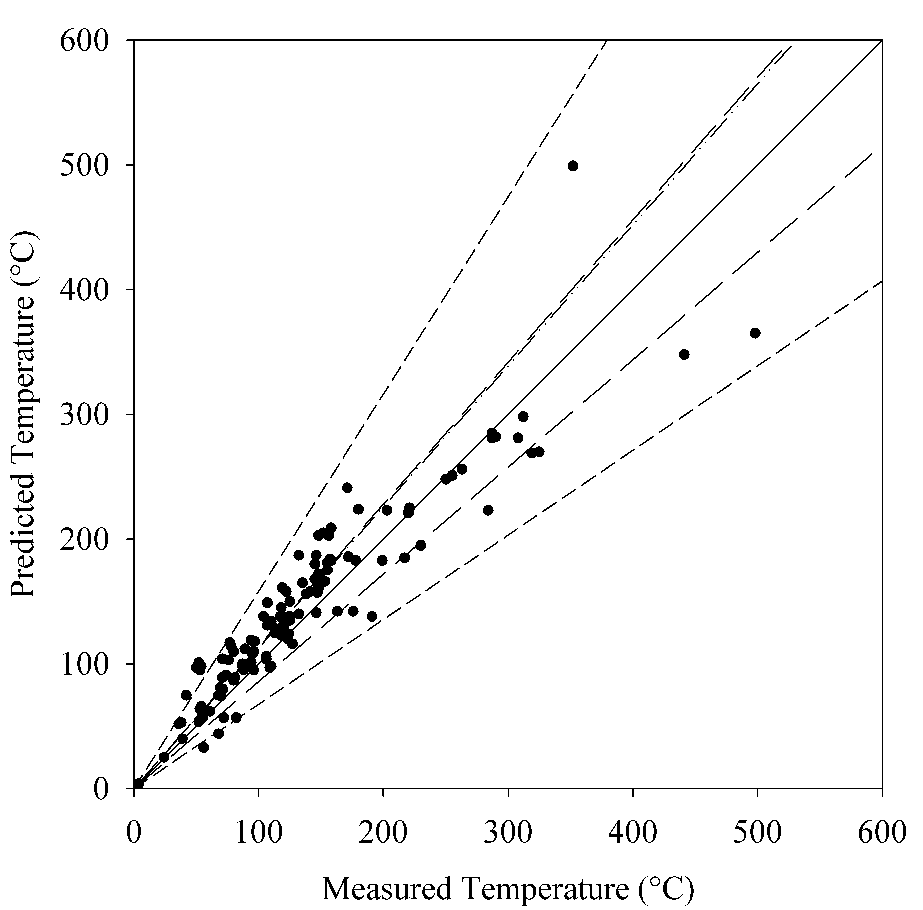
\includegraphics[width=3.2in]{Fig_scatter_plot}
\caption{A comparison of measured versus predicted wall temperature. The off-diagonal lines indicate the $2 \widetilde{\sigma}$ bounds for the experiments (long dash) and the model (short dash).}
\label{scatterplot}
\end{figure}
The accuracy of the model can be expressed in terms of two statistical parameters. The first, $\delta$, is the bias factor. It indicates the extent to which the model, on average, under or over-predicts the measurements. For example, the bias factor for the data shown in Figure~\ref{scatterplot} is 1.13. This means that the model over-predicts wall temperatures by 13~\%, on average, and this is shown graphically by the dash-dot line. The second statistic is the relative standard deviation of the model, $\widetilde{\sigma}_M$. This indicates the degree of scatter of the points. Referring again to Figure~\ref{scatterplot}, there are two sets of off-diagonal lines. The first set, shown as long-dashed black lines, indicate the estimated experimental uncertainty. The slopes of these lines are $1\pm 2 \widetilde{\sigma}_E$, {\em i.e.} the 95~\% confidence interval for the measurements. In this case, $\widetilde{\sigma}_E=0.07$. The second set of off-diagonal lines, shown as short-dashed lines, indicates the model uncertainty. The slopes of these lines are $\delta (1\pm 2 \widetilde{\sigma}_M)$. In this case, $\widetilde{\sigma}_M=0.2$. If the model were as accurate as the measurements against which it is compared, the two sets of off-diagonal lines would merge and the dash-dot bias line would overlap the solid diagonal line. The extent to which the data scatters outside of the experimental bounds is an indication of the degree of model uncertainty.

The derivation of these uncertainty statistics is described in Ref.~\cite{McGrattan:Metrologia}, and it is summarized here. First, a few assumptions are made:
\begin{enumerate}
\item The experimental measurements are assumed to be unbiased, and their uncertainty is assumed to be normally distributed with a constant relative standard deviation, $\widetilde{\sigma}_E$.
\item The model uncertainty is assumed to be normally distributed about the predicted value divided by a bias factor, $\delta$. The relative standard deviation of the distribution is denoted as $\widetilde{\sigma}_M$.
\end{enumerate}
Now, given a set of experimental measurements, $E_i$, and a corresponding set of model predictions, $M_i$, compute the following:
\begin{equation}
   \overline{\ln (M/E)} = \frac{1}{n} \, \sum_{i=1}^n \, \ln (M_i/E_i)
\end{equation}
The relative standard deviation of the model, $\widetilde{\sigma}_M$, can be computed from the following equation:
\begin{equation}
   \widetilde{\sigma}_M^2 + \widetilde{\sigma}_E^2 = \frac{1}{n-1} \sum_{i=1}^n \,
   \left[ \ln (M_i/E_i) - \overline{\ln (M/E)}  \right]^2 \label{stdev}
\end{equation}
The bias factor is:
\begin{equation}
   \delta = \exp \left( \overline{\ln (M/E)} + \frac{ \widetilde{\sigma}_M^2}{2}-\frac{\widetilde{\sigma}_E^2}{2} \right) \label{delta}
\end{equation}
For a given model prediction, $M$, the ``true'' value of the quantity of interest is assumed to be a normally distributed random variable with a mean $\mu=M/\delta$ and a standard deviation of $\sigma=\widetilde{\sigma}_M (M/\delta)$.
Using these values, the probability of exceeding a critical value, $x_c$, is:
\begin{equation}
   P(x>x_c) = \frac{1}{2} \; \hbox{erfc} \left( \frac{x_c-\mu}{\sigma \sqrt{2}} \right) \label{prob}
\end{equation}
Note that the complimentary error function is defined as follows:
\begin{equation}
   \hbox{erfc}(x) = \frac{2}{\sqrt{\pi}} \int_t^\infty e^{-t^2} dt
\end{equation}
It is a standard function in most mathematical or spread sheet programs.

As an example of the procedure, suppose that the model whose results are plotted in Figure~\ref{scatterplot} has predicted that the wall temperature within a compartment would peak at a value of 300~$^\circ$C due to a given design fire. Suppose also that the failure criterion for the wall lining material is 325~$^\circ$C. What is the probability that the wall temperature could reach 325~$^\circ$C? First, it is best to work in terms of temperature rise. The ambient temperature is 20~$^\circ$C; thus, the predicted temperature rise, $\Delta T_p$, is 280~$^\circ$C and the critical temperature rise, $\Delta T_c$, is 305~$^\circ$C. From Equation~\ref{prob}, the probability that the temperature could exceed the critical value is:
\begin{eqnarray}
   P(\Delta T>\Delta T_c) &=& \frac{1}{2} \; \hbox{erfc} \left( \frac{\Delta T_c-(\Delta T_p/\delta)}{\widetilde{\sigma}_M \, (\Delta T_p/\delta) \sqrt{2}} \right) \nonumber \\ [0.1in]
    &=& \frac{1}{2} \; \hbox{erfc} \left( \frac{305-(280/1.13)}{0.2 \; (280/1.13) \, \sqrt{2}} \right) \cong 0.12
\end{eqnarray}
It must be emphasized that this estimated probability of failure is based only on the model uncertainty. It does not account for parameter uncertainty; that is, the uncertainty in the input parameters.



\section{Applications}

This section presents examples of how CFD fire models are used in practice. These applications can be divided into three general categories -- research, design, and forensic. For research, the models can help explain basic fire phenomena. For design, the models are used to predict the spread of smoke and heat from a hypothetical fire in a real or planned building. For forensics, the models aid in the reconstruction of an actual fire. For a design application, the fire is usually specified; that is, the ignition, growth, and eventual decay of the fire are not predicted by the model but rather specified by the design engineer and reviewed by the code enforcing authority. For a reconstruction, the model is usually used to explain how a small fire grew and spread to cause serious damage or injury. Rarely are fire models of the type described in this chapter used to show how a fire was actually ignited, as the physical mechanism of this event (electrical short, arcing fault, arson, etc.) is usually not included in the model.

\subsection{Fundamental Fire Dynamics}

CFD, in particular large eddy simulation, provides a convenient means to study basic fire behavior. The most obvious application is the study of fire plumes; for example, predicting the height of the visible flame, the centerline velocity and temperature, and the pulsation frequency. Heskestad's empirical flame height correlation (Equation~\ref{Heskestad_Flame_Height}) is valid for values of  $Q^*$ between 0.1 and 10,000, characterizing intermittent grass fires all the way to oil well blowout fires. Figure~\ref{Flame_Height} compares FDS predictions with Heskestad's correlation. Note that the simulations were run at three different grid resolutions. A useful way to characterize the grid resolution of a fire simulation is via the ratio $D^*/\delta x$, where $D^*$ (Equation~\ref{Dstar}) is a measure of the effective fire diameter, based on heat release rate, and $\delta x$ is the size of a grid cell. In effect, $D^*/\delta x$ is the number of grid cells spanning the effective fire diameter.
\begin{figure}[ht]
\begin{center}
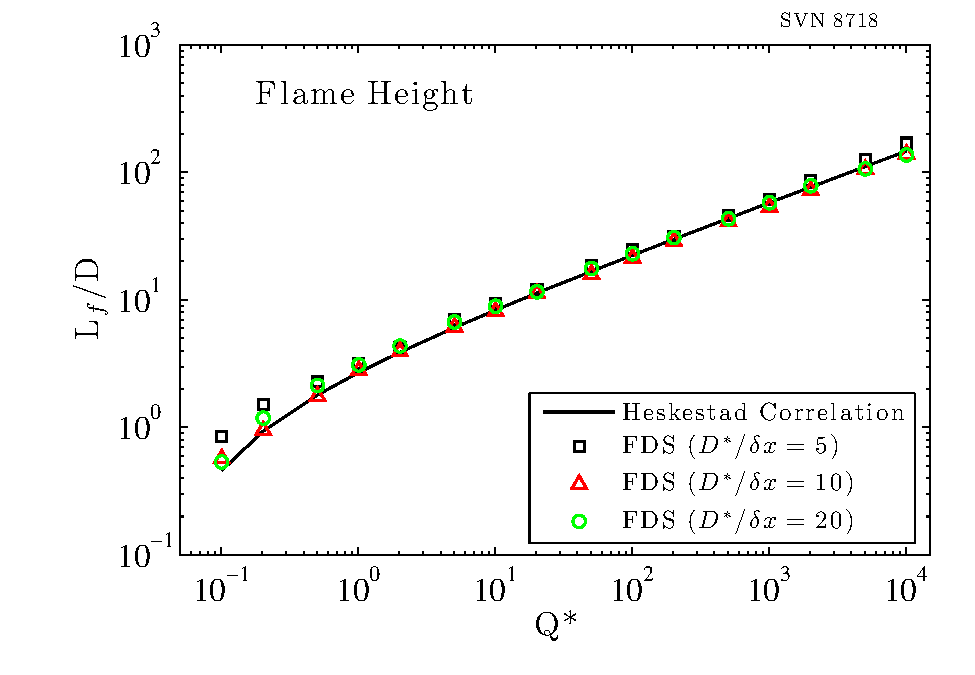
\includegraphics[width=4.0in]{Fig_flame_height}
\end{center}
\caption{Comparison of FDS predictions of flame height from a 1~m square pan fire for Q* values ranging from
0.1 to 10000.}
\label{Flame_Height}
\end{figure}

The fundamental, or ``puffing,'' frequency is a quantity that the fire model also ought to predict accurately. Figure~\ref{Sandia_Simulation} displays sequential flame images for a single puff from a simulation of a 1~m methane fire experiment conducted at Sandia National Laboratories~\cite{Tieszen:2002}. The dominant puffing mode shows good agreement with the measured puffing frequency of 1.65~Hz. Higher frequency fluctuations from the simulation exhibit the classic -5/3 scaling of Kolmogorov turbulence~\cite{Pope:2000}.
\begin{figure}[ht]
\begin{center}
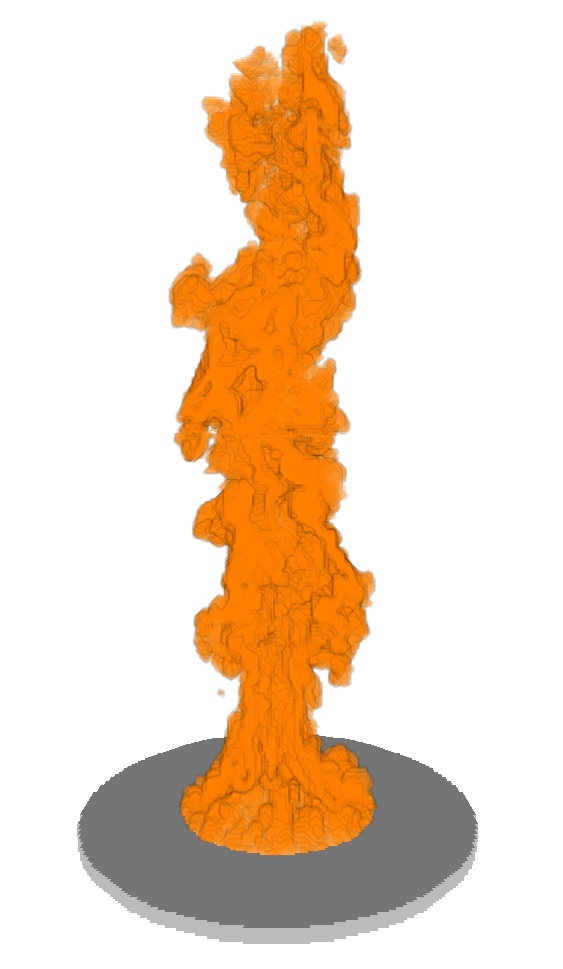
\includegraphics[width=1.2in]{Fig_fire_1}
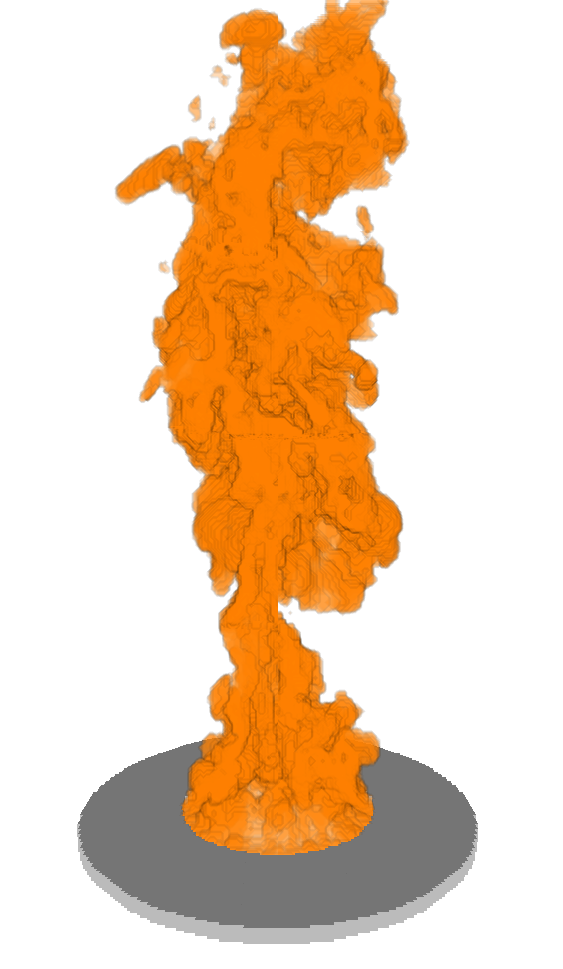
\includegraphics[width=1.2in]{Fig_fire_2}
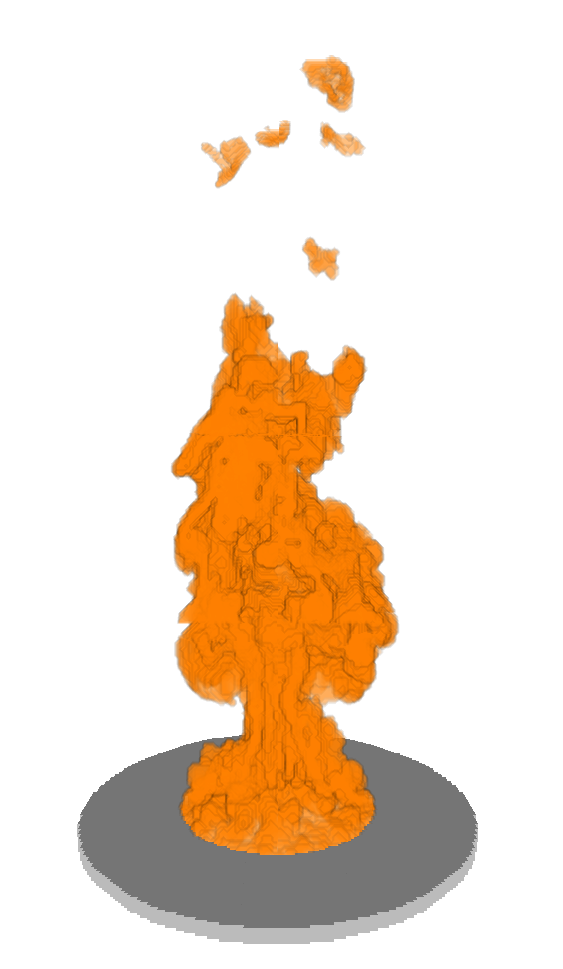
\includegraphics[width=1.2in]{Fig_fire_3}
\end{center}
\caption{Snapshots of the flame envelope from a simulation of the Sandia 1~m diameter methane pool fire using 1.5~cm grid resolution.  The images span a single ``puff''.}
\label{Sandia_Simulation}
\end{figure}



\subsection{Smoke Movement}

A significant proportion of fire fatalities can be attributed to the inhalation of smoke particulates and toxic gases. Furthermore, the effects of reduced visibility, high temperature, radiative flux, and oxygen depletion may add to the hazard associated with the smoke generated by an enclosure fire. Means to control the movement of smoke include physical barriers, natural or mechanical smoke exhaust, and pressurization of protected spaces. In routine applications, the design of the smoke control measures may often be achieved by recourse to various guidance publications and empirical correlations~\cite{Klote, NFPA:92B}. Network airflow and zone fire models are also available to assist in the design process. However, where the building space is large or complex in shape, or where a novel ventilation system is proposed, CFD can be a useful tool. Covered shopping malls, atria in hotels and office buildings, leisure complexes, airport terminals, and large warehouses are just some examples of where CFD is being increasingly employed.

Many  of  the  earliest  examples  of  the  application of CFD to fire engineering were in smoke movement applications~\cite{Pericleous, Cox:1990}. Simulations were at that time restricted to a few tens of thousands of grid cells. Although this number has increased to hundreds of thousands or even millions of cells, many of the modeling issues remain the same and are discussed later~\cite{Kumar}.




\paragraph{Smoke transport in a historic landmark}

CFD fire modeling is commonly used during the renovation of historic buildings. Often at issue is the inclusion or exclusion of a fire protection system (sprinklers, exhaust fans, etc.) that might require a variance from the local building code requirements. For example, as part of an overall effort in modernizing the Rhode Island Statehouse (the rotunda is the fourth largest self-supporting dome in the world), the LES model FDS was used to model a number of fire scenarios within the structure. The building supervisors wished to avoid having to disrupt the historical fabric of the rotunda while updating the building's fire protection systems. The model was used to examine a number of fire scenarios and how they might impact the ability of occupants to evacuate the building. Note in Figure~\ref{Dome} the use of rectangular obstructions to approximate the very complicated geometry of the building -- a simple alternative to the more CPU intensive body-fitted coordinate system.

\begin{figure}[ht]
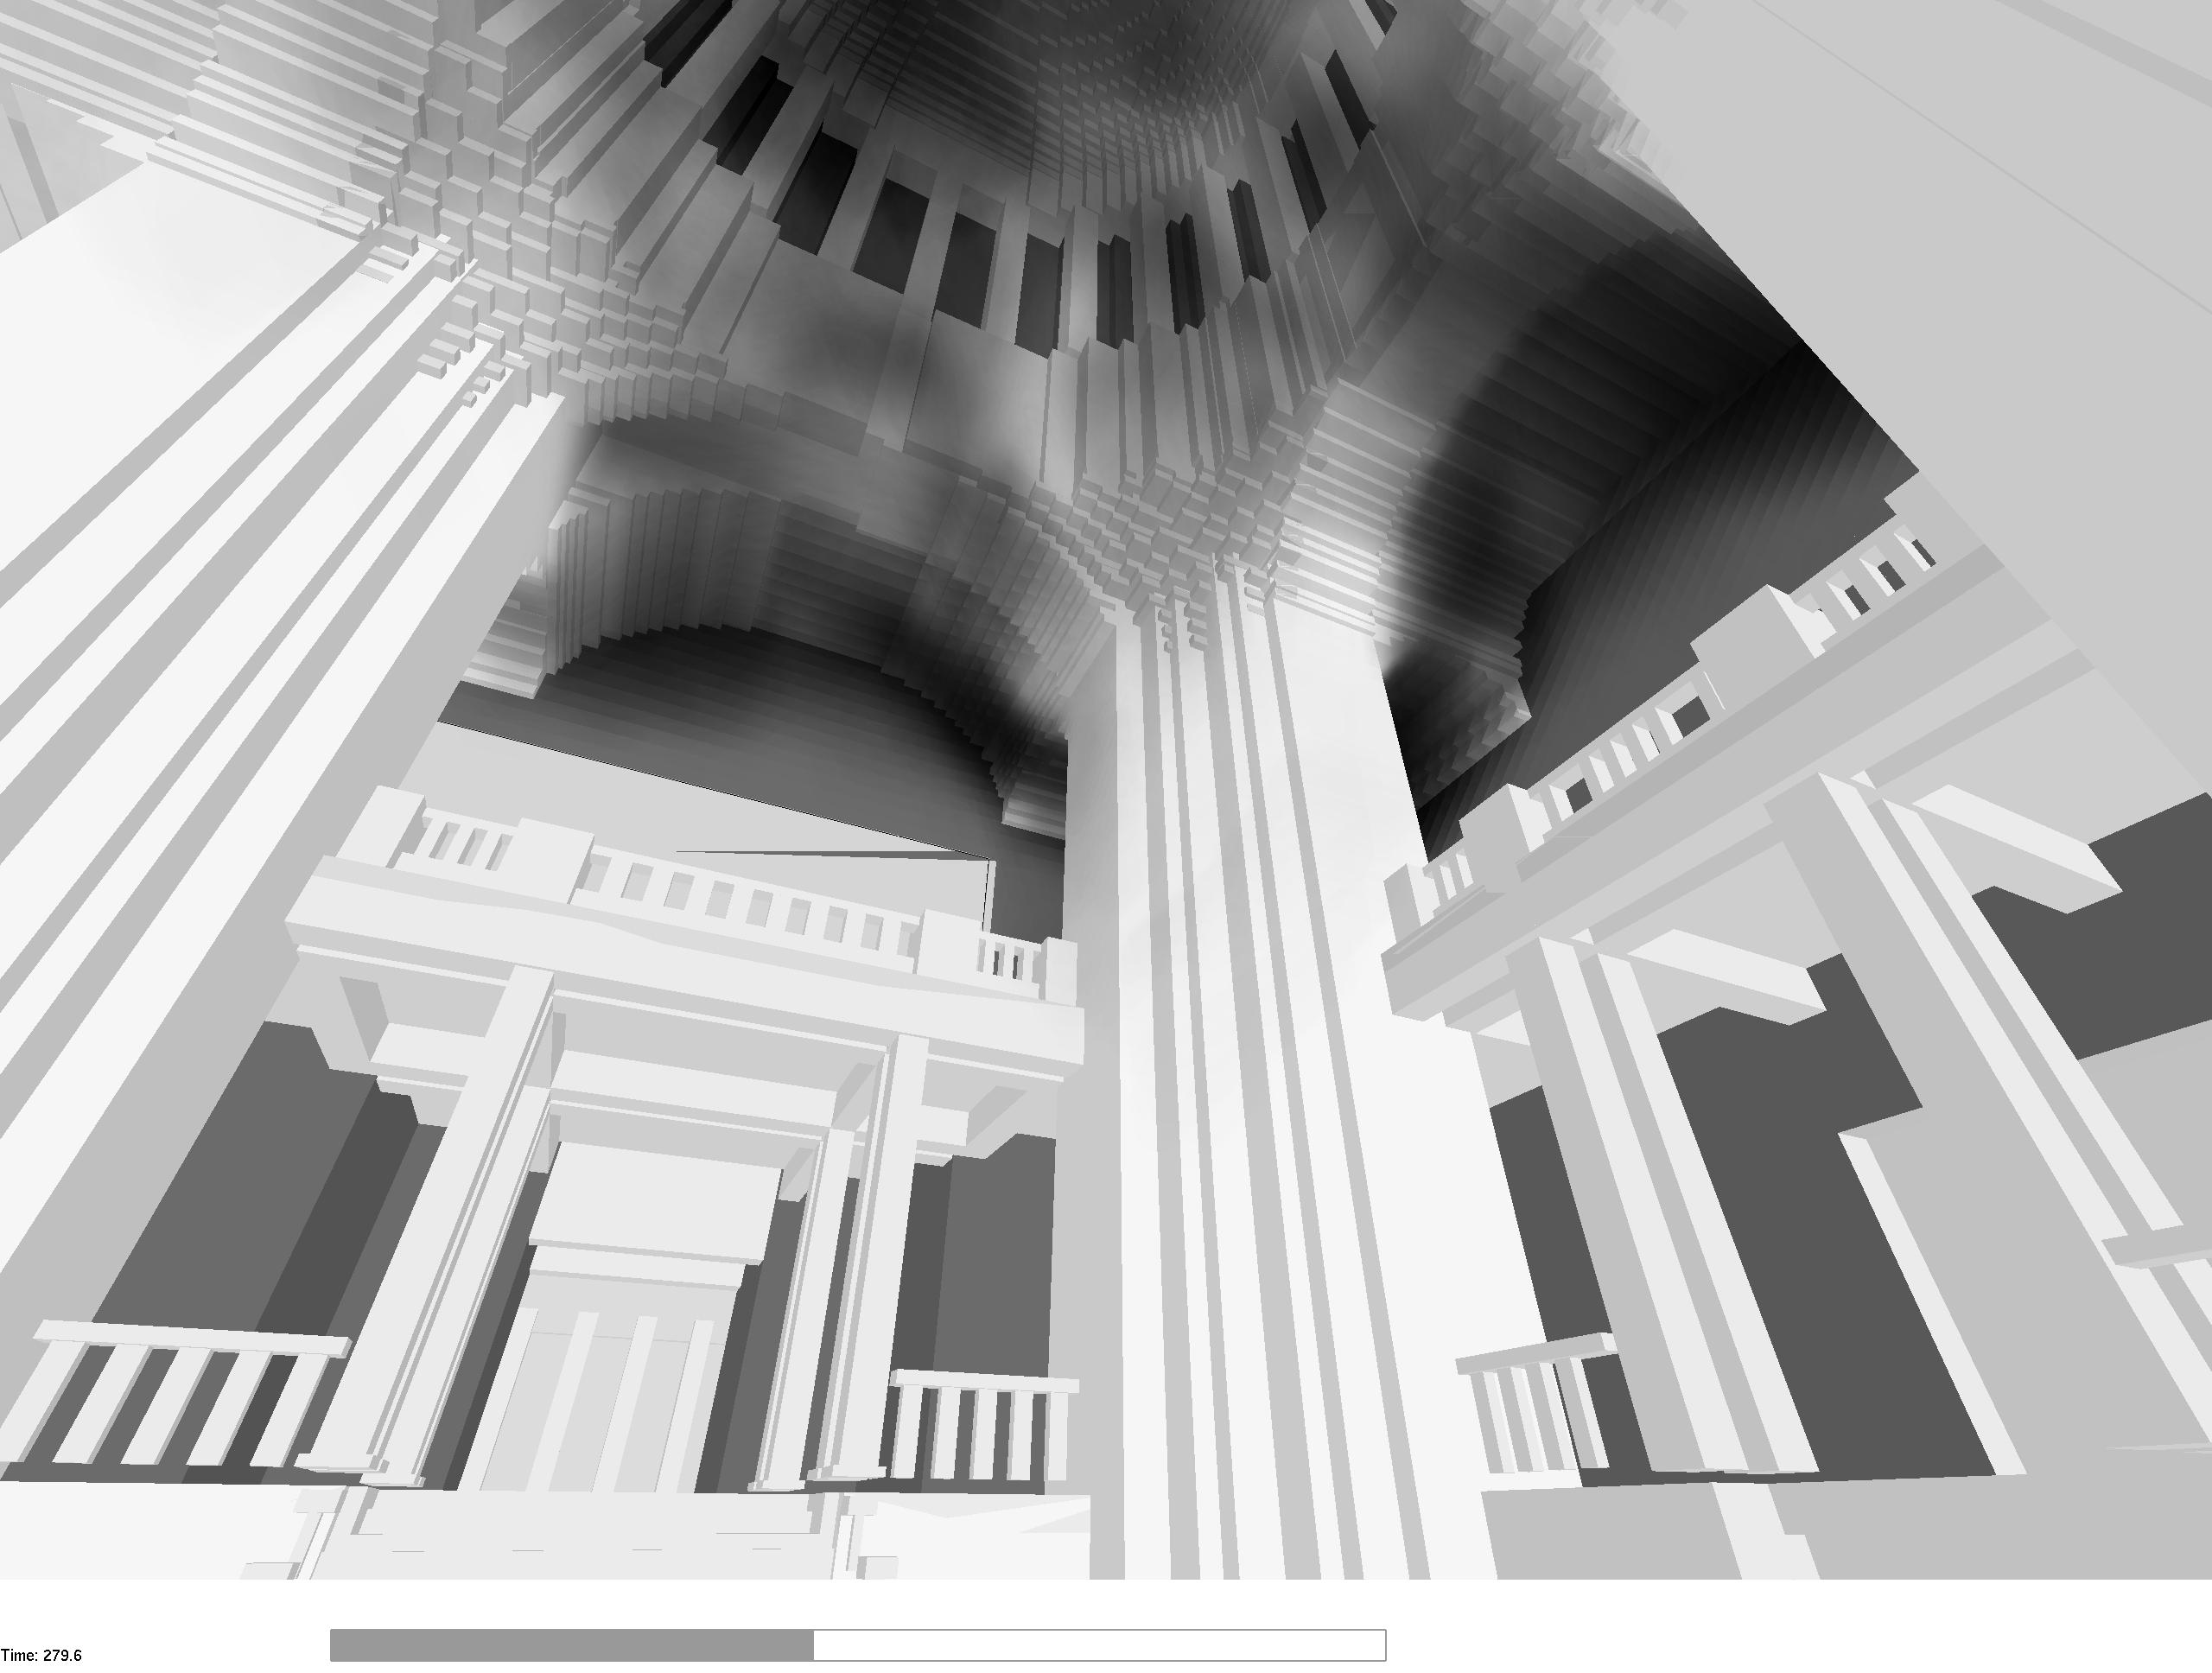
\includegraphics[width=\textwidth]{Fig_dome}
\caption{Smoke filling analysis of the Rhode island State capitol. (Figure courtesy Hughes Associates.)}
\label{Dome}
\end{figure}




\paragraph{Smoke transport in a multistory residential building}

To assist means of escape and fire fighter access in high rise residential buildings it is common practice to provide some form of smoke control to the stairwells, which could take the form of a sophisticated pressurization scheme or a relatively simple natural ventilation provision. There may be cases where smoke protection is required also in the corridors and lobbies at each story, possibly as a compensatory measure for extended travel distances. Another approach, adopted in some parts of the world, is to provide mechanical ventilation in the corridor. In the event of a fire in an adjoining apartment smoke is purged from the corridor, while at the same time the ventilation system provides smoke protection to the stairwell by the combined action of pressure differentials and open-door airflows akin to a stair pressurization system. CFD modeling of the air and smoke transport in the corridor and stairwell is often required in support of the design, in particular where the corridors and lobbies have a more complicated layout or the ventilation inlets and outlets cannot be installed in ideal locations.



\paragraph{Tunnels}

Historically, smoke control inside tunnels was often considered as an afterthought to design of ventilation for the provision of fresh air. Where natural ventilation was insufficient, mechanical ventilation was designed using network flow theory aided in recent years by network models. As a two-layer description is generally not valid within a tunnel environment, fire zone models have been applied to tunnels in only a limited number of cases. CFD, however, is now finding increasing application to fire hazard analysis for road tunnels in particular. In recent years a number of major tunnel fire incidents such as the tragedy in the Mont Blanc tunnel in 1999, resulting in 39 deaths, have highlighted the need to understand better the mechanism of fire development and spread inside tunnels. In particular, heat transfer to the tunnel walls is important to account for correctly as this has a strong influence on the distribution of heat along the tunnel, the degree of stratification that can be expected, and the threat to the integrity of the structure.

One area where CFD has been applied successfully is in the analysis of the critical velocity required in a longitudinally ventilated tunnel to control the spread of heat and smoke so that it is forced in the downstream direction, providing safe conditions upstream~\cite{Hwang}. Another area currently receiving much attention is the choice of design fire for tunnel fire safety design. In the light of the recent tunnel fire incidents and full-scale fire tests~\cite{Ingason}, the size of the fire load that can be generated from what were previously considered as nonhazardous cargoes has been revised. Heat release rates well in excess of 100~MW have been measured for heavy-goods vehicles carrying commercial merchandize.

CFD was used in the investigation into the Mont Blanc tunnel fire incident in 1999. One of the modeling studies involved the use of the JASMINE fire model to re-construct conditions inside the tunnel during the first 30~minutes, during which time most of the fatalities would have occurred. Using information available on the ventilation settings and the location of vehicles, the model predicted the transport of smoke and heat along the length of the tunnel. The data were then fed into a model for fractional effective dose to enable an assessment of when and how the fatalities occurred. Subsequent parametric simulations were performed to investigate whether alternative tunnel ventilation measures would have helped on the day of the incident~\cite{Miles:2004}.


\paragraph{Parking Garages}

The application of CFD to the analysis and design of smoke control systems in basement car parks may share elements that apply also to road tunnels. Not only is the potential fire source similar, the ventilation strategies and performance criteria may well overlap. Two ventilation strategies that might be considered in a basement car park include dilution (purging by fresh air) and the directional control of smoke by the application of applied air flows.

While diluting smoke and vehicle emissions can in principle be achieved by ventilating at a specified air change rate, in many cases additional ventilation provisions will be required in order to ensure an even mixing of fresh air and the elimination of stagnant regions. This is commonly achieved by the strategic location of impulse (jet) fans on the underside of the ceiling, which assist the movement of air from the inlet points to the exhaust locations. CFD may be usefully employed to determine the number and location of these fans.

The directional control of smoke in the event of a fire, with the objective of providing a relatively smoke free access to the location of the fire for fire fighting personnel, presents a greater challenge than simply purging smoke from the car park. Here careful design of the ventilation system is required, with the impulse fans operating akin to the case of a longitudinally ventilated tunnel, directing the smoke and heat in a direction away from the approaching personnel.



\subsection{Fire Investigation}

CFD is increasingly used to reconstruct  actual  fires,  providing  fire  service  personnel and fire investigators with a better understanding of the events that led to injury, loss of life, or loss of the structure. In any reconstruction, the time line of events provided by the first responders and other eyewitnesses is as crucial as the model input, but it is also invaluable in assessing the results. Rendering the results of the simulation as realistically as possible facilitates the synthesis of model simulation with photographic and visual evidence. Most people at the fire scene are certainly not experts in CFD, but they are very experienced with fire. Examples of how CFD has been used in actual fire reconstructions are available~\cite{Grosshandler, McGrattan:2005, Madrzykowski:2000, Madrzykowski:2004, Christensen}.

As an example, NIST researchers used the Fire Dynamics Simulator to analyze a fire that occurred on the evening of June 18, 2007, in a furniture store in Charleston, South Carolina~\cite{Bryner:2011}. Using evidence collected at the scene and eyewitness accounts, the investigators put together a plausible sequence of events that led to the deaths of nine fire fighters. Figure~\ref{furniture_store} presents a snapshot of the numerical simulation compared to a photograph of the actual fire.
\begin{figure}[ht]
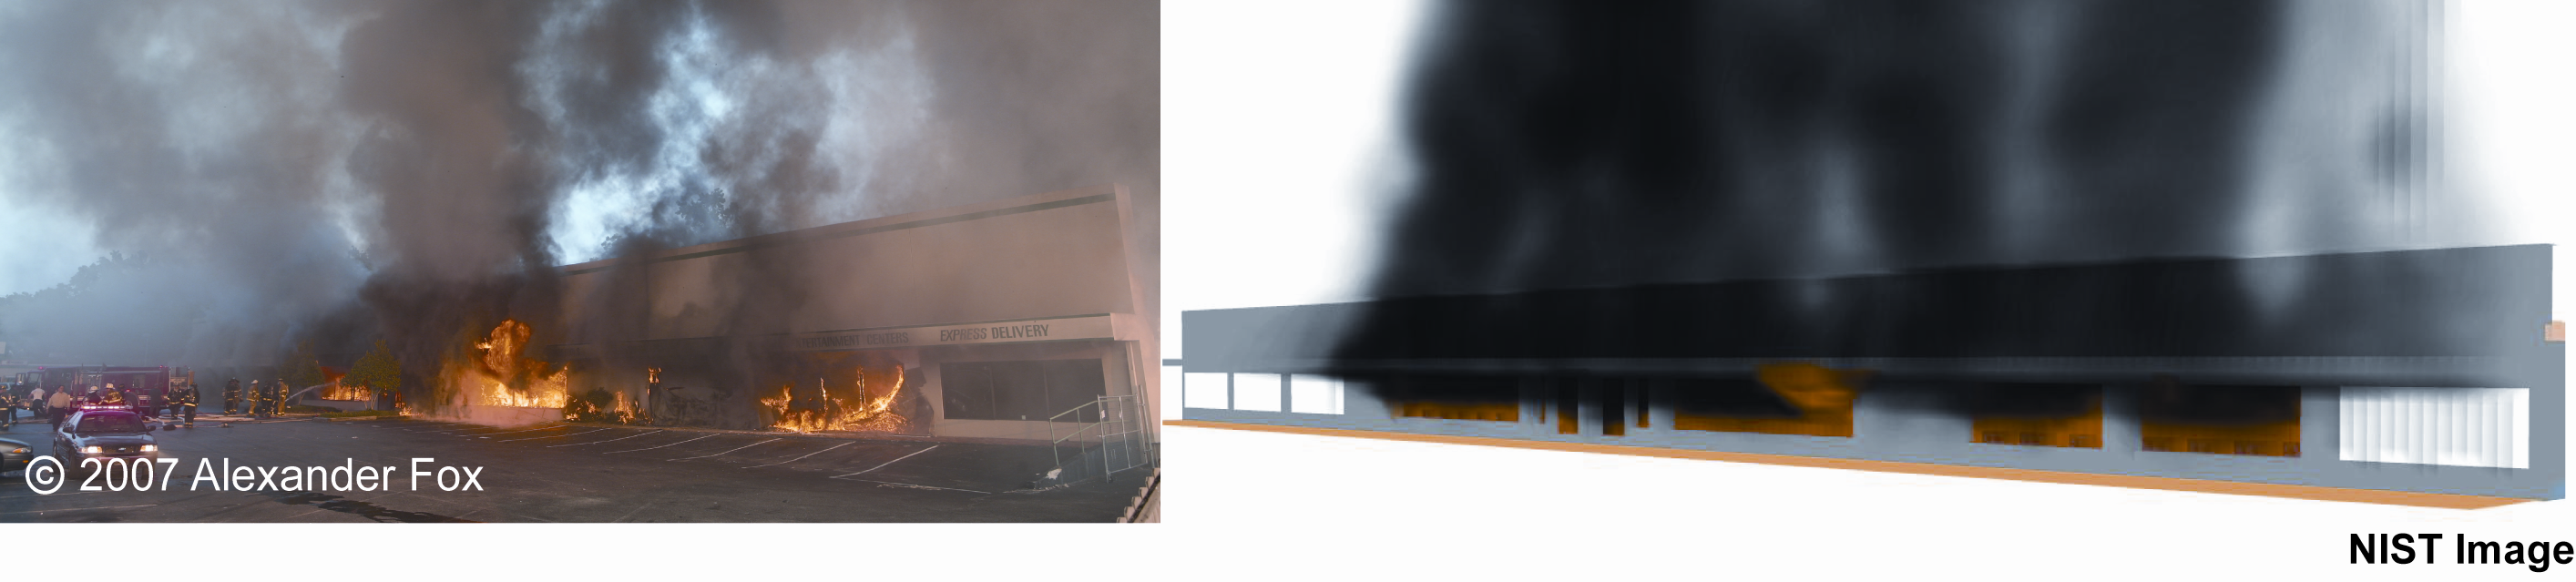
\includegraphics[width=\textwidth]{Fig_store_fire}
\caption{Comparison of photographs of the Charleston furniture store fire with a numerical simulation. Figure courtesy of NIST.}
\label{furniture_store}
\end{figure}



\subsection{Outdoor Applications and Wind}

Buoyant windblown plumes have been studied since the early 1960s. A summary of the early work together with a useful bibliography is given by Turner~\cite{Turner}. Most of the models described in these works are integral models, where the profiles of physical quantities in cross-sectional planes perpendicular to the wind direction are assumed, together with simple laws relating entrainment into the plume to macroscopic features used to describe its evolution.

The potential shortcomings of these types of models are that they were designed for typical industrial sources, like smokestacks, that are much smaller in terms of energy output than a large fire. The plume from an oil or forest fire will rise higher into the atmosphere, and it is difficult to predict the rise based on empirical correlations. If the plume rise is not calculated correctly, substantial errors in downwind concentration can result. In the case of smoke-stack emissions, the plume does not rise appreciably high, reducing the uncertainty of the results.
Most of the assumptions required by integral models can be removed by taking advantage of the advances in CFD over the past few decades. For example, as part of the process of evaluating the feasibility of using in situ burning as a remediation tool for large oil spills, NIST developed a numerical model, ALOFT (A Large Out- door Fire plume Trajectory), to predict the concentration of smoke and other combustion products downwind of a large fire~\cite{Baum}. The model is simply a variant of the large eddy simulation model FDS, with a simplified plume rise model coupled with a coarsely gridded wind calculation spanning tens of kilometers (Figure~\ref{ALOFT}). This combination of models is not unusual for outdoor application, as the range of length scales spans at least three orders of magnitude.

\begin{figure}[ht]
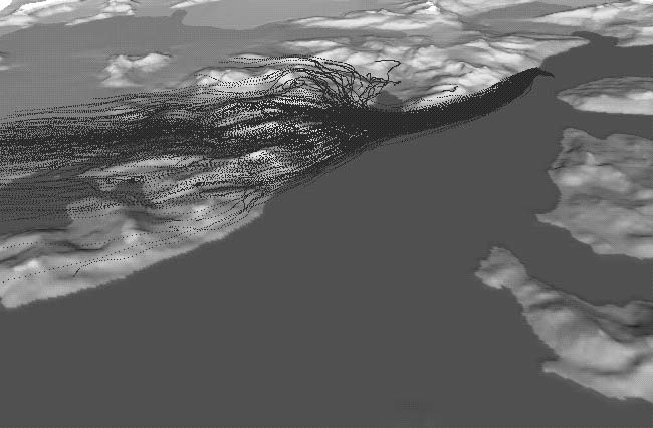
\includegraphics[width=\textwidth]{Fig_outdoor_plume}
\caption{Simulation of smoke from a large oil fire in the Valdez narrows, Alaska. (Figure courtesy of NIST.)}
\label{ALOFT}
\end{figure}



\subsection{Virtual Experiments}

Many codes and standards for fire protection are based upon simple room geometries. For example, the spacing for smoke detectors has historically been based upon smooth, level ceilings with some additional rules for beams, slope, and height.  Under those rules a single story room with a 30~m by 30~m smooth ceiling could be protected by a grid of nine smoke detectors, but a ceiling of waffle concrete construction (Figure~\ref{waffle_ceiling}) with structural deep beams 1~m on center, could, under a strict interpretation of the guidelines, require 900 detectors, one in each beam pocket. While this is obviously unreasonable, making a change to the building code requires evidence. In lieu of a large number of costly full-scale experiments, a small set of full-scale experiments was combined with a large set of ``virtual'' experiments done with CFD~\cite{O'Connor:NFPRF,Mealy:NFPRF}.
\begin{figure}[ht]
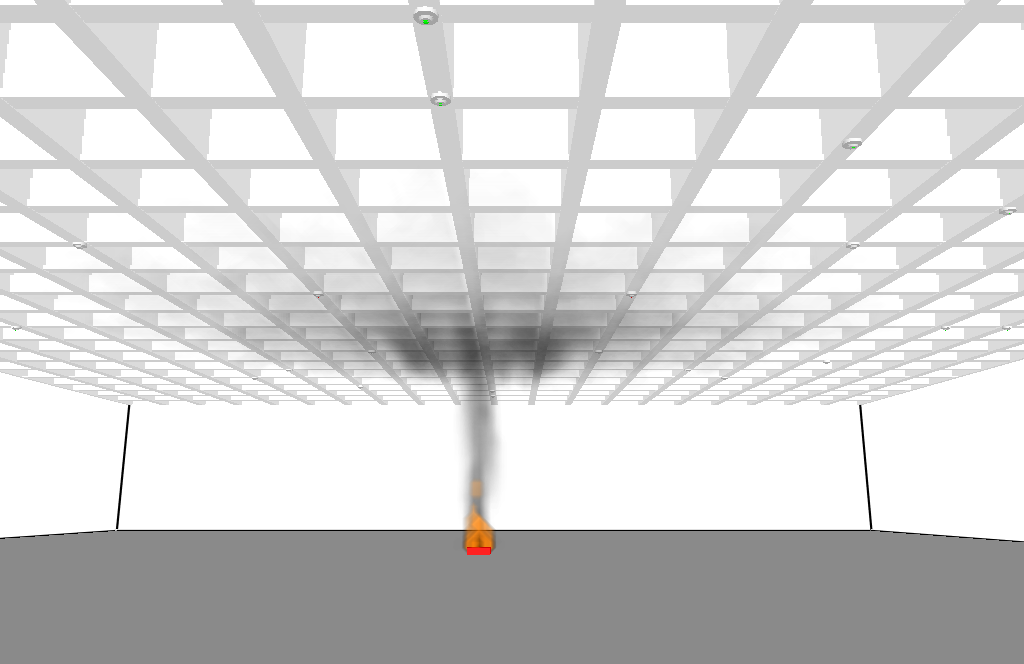
\includegraphics[width=\textwidth]{Fig_waffle_ceiling}
\caption{Simulation of smoke filling under a coffered ceiling. (Figure courtesy Aon Fire Protection Engineering Corp.)}
\label{waffle_ceiling}
\end{figure}
The researchers evaluated the appropriateness of the prescriptive provisions and identified ceiling structure parameters, which if altered, would cause significant differences in smoke detection performance as compared to a smooth level ceiling. It had been believed that such beam projections would significantly delay the activation time. The use of CFD modeling showed this expectation to be incorrect and a subsequent full-scale experimental study proved the general findings of the CFD analysis~\cite{Gottuk:2008}. The final result of the study led to an exception, under some circumstances, to the code requirement of a smoke detector in every beam pocket.


\section{The Role of CFD in the Design Process}

As discussed elsewhere in this chapter, CFD has an ever increasing role to play in the development of fire safety science, and has an important contribution to make in better understanding the fundamentals such as flame spread and chemical species production where it is being used in parallel with physical experiments. However, it is as a fire engineering design tool that CFD is probably of most relevance to the majority of readers. Here a few words of caution are worth noting.

CFD modeling has a useful, and sometimes critical, role in developing safe and robust fire engineering solutions where the control of smoke and heat generated by fire forms part of the fire safety strategy. It allows architectural designs to be adopted that in previous eras would have been difficult to justify, for example in respect to smoke control in large and complicated building atria or where a reduced level of structural fire protection is desired. It should, however, be seen as a contributing component to the overall design process, and not as a ``black box'' that faithfully provides the correct answers regardless of the inputs and assumptions made. A great deal of care and experience is required in order to sensibly use CFD in support of fire engineering designs, and it should be employed alongside simpler calculation and design methods wherever possible to confirm that the CFD results are comparable to the empirical correlations that have traditionally been applied in fire protection engineering.

It is as a parametric design tool that CFD is often most gainfully employed, allowing the impact of varying the input and boundary conditions to be examined. For example, how sensitive is the smoke control solution to the design fire size, or how much influence does a change in wind direction have on a natural smoke ventilation strategy? The reader is encouraged to consult the guidance documents available on the best practice use of CFD in the various application areas and to consult the guidance documentation provided with the CFD model being employed. For example, the guidance document prepared by the U.S.~Nuclear Regulatory Commission and the Electrical Power Research Institute (EPRI) on fire modeling for nuclear power plants~\cite{Stroup:2012} includes useful information on the appropriate role and application of CFD in the fire safety design process, and is relevant also to fire scenarios outside the nuclear field.




\section{Summary}

Computational fluid dynamics modeling of fire has made tremendous progress over the past few decades as our understanding of fire improves and as computers get ever faster. However, although it appears to many that CFD is the cutting edge of fire protection engineering, many non-modelers are surprised to learn that our ability to reproduce fire phenomena via computer simulation lags our empirical understanding by about 10 years. Indeed, current-generation models address transport phenomena reasonably well, making them useful for many engineering applications. However, they have not yet reached the point of reliably predicting, for large-scale applications, such important phenomena as flame spread, extinction, suppression, and CO and smoke production, all of which demand more detailed chemistry and physics than are currently incorporated in the models.

Moving forward will require a new generation of engineers who have expertise in fire physics, mathematics, and computer science to build on the knowledge possessed by the current generation of modelers. This chapter sets forth the basic elements to lay the foundation of further study for future modelers, and it also provides the current practitioner with a better understanding of the models being used.



\section{Nomenclature}

\begin{tabbing}
$c_p$ 	\hspace{1in}     \= specific heat \\
$D_\alpha$	             \> material diffusivity of species $\alpha$ \\
$\mathbf{f}$	         \> external body force \\
$h_{\rm s}$              \>	sensible enthalpy \\
$h_{\rm c}$ 	         \> convective heat transfer coefficient \\
$I$	                     \> radiant intensity \\
$k$	                     \> thermal	conductivity; turbulent	kinetic energy \\
$\dot{m}_\alpha'''$      \> mass production (destruction) rate of species $\alpha$ per unit volume \\
$p$	                     \> pressure \\
Pr	                     \> Prandtl number \\
$\dot{\mathbf{q}}''$	 \> heat flux vector \\
$\dot{q}''$              \> heat release rate per unit area \\
$\dot{q}'''$             \> heat release rate per unit volume \\
$\cal R$                 \> universal gas constant \\
$\mathbf{s}$	         \> direction vector \\
$s$	                     \> stoichiometric air requirement of the fuel \\
$S_{ij}$ 	             \> strain tensor \\
Sc	                     \> Schmidt number \\
$t$	                     \> time \\
$T$	                     \> temperature \\
$\mathbf{u}=(u,v,w)$     \> velocity vector \\
$\overline{W}$	         \> average molecular weight \\
$\mathbf{x}=(x,y,z)$	 \> position vector \\
$Y_\alpha$               \> mass fraction of species $\alpha$
\end{tabbing}

\subsection{Greek Letters}

\begin{tabbing}
$\epsilon$ \hspace{1in}  \= rate of dissipation of turbulent kinetic energy \\
$\kappa$                 \> radiation absorption coefficient \\
$\lambda$                \> generalized diffusion coefficient \\
$\mu$                    \> dynamic viscosity \\
$\mu_t$                  \> turbulent viscosity (in eddy viscosity turbulence model) \\
$\rho$                   \> density \\
$\sigma$                 \> Stefan-Boltzmann constant \\
$\tens{\tau}$	         \> stress tensor
\end{tabbing}


\bibliographystyle{unsrt}
\bibliography{CFD_Modeling_Chapter}

\section*{Appendix}
\addcontentsline{toc}{section}{Appendix}

Much of the difficulty in learning and applying computational fluid dynamics is the complexity of the governing equations. In this Appendix, some of the common terms found in the mass, momentum, and energy equations are expanded. Many of the variables and operators can be represented as $3 \times 3$, $1 \times 3$, or $3 \times 1$ matrices, and the expansions can be carried out following the rules of linear algebra. For example, the divergence of the flow vector, $\nabla \cdot \mathbf{u}$, is a scalar formed by multiplying the $1 \times 3$ gradient operator $\nabla$ and the $3 \times 1$ vector $\mathbf{u}$. On the other hand, the product of the velocity vectors, $\mathbf{u} \mathbf{u}$, is found by multiplying a $3 \times 1$ vector by a $1 \times 3$ vector:
\begin{equation}
\mathbf{u}\mathbf{u} = \left( \begin{array}{c} u \\ v \\ w \end{array} \right) (u,v,w) = \left( \begin{array}{ccc} u^2 & uv & uw \\ vu & v^2 & vw \\ wu & wv & w^2 \end{array} \right)
\label{matmult}
\end{equation}
Thus, the convection term in the momentum conservation equation can be expanded as follows:
\begin{eqnarray}
\nabla \cdot (\rho \mathbf{u}\mathbf{u})
&=& \left( \frac{\partial}{\partial x} \; \frac{\partial}{\partial y} \; \frac{\partial}{\partial z} \right)
    \left( \begin{array}{ccc} \rho u^2 & \rho uv & \rho uw \\ \rho vu & \rho v^2 & \rho vw \\ \rho wu & \rho wv & \rho w^2 \end{array} \right) \nonumber \\
&=& \left( \begin{array}{c} (\rho u^2)_x + (\rho vu)_y + (\rho wu)_z \\ (\rho uv)_x + (\rho v^2)_y + (\rho wv)_z \\ (\rho uw)_x + (\rho vw)_y + (\rho w^2)_z \end{array} \right)^T
\end{eqnarray}
The result is a vector whose components form the convective terms of the three component momentum equation. Note that here the subscripts $x$, $y$, and $z$ denote partial derivatives with  respect to that particular coordinate direction.

The term for the viscosity in the momentum equation, $\nabla \cdot \tens{\tau}$, is deceptively simple. In reality, it is not, and because it constitutes the heart of the debate over turbulence models, some attention must be paid to it. Using customary tensor notation, the viscous stress tensor is defined as
\begin{equation}
\tens{\tau}_{ij} = \mu \left( \frac{\partial u_i}{\partial x_j} + \frac{\partial u_j}{\partial x_i} - \frac{2}{3} \delta_{ij} \nabla \cdot \mathbf{u} \right) \quad ; \quad \delta_{ij} = \left\{ \begin{array}{l} 1 \; \mathrm{if} \; i=j \\ 0 \; \mathrm{if} \; i\neq j \end{array} \right.
\end{equation}
These expressions assert that the viscous stresses are linearly related to the strains, the very definition of a Newtonian fluid. The proportionality constant, $\mu$, is called the dynamic viscosity of the fluid. The viscous stress tensor can also be represented as a $3 \times 3$ matrix:
\begin{equation}
\tens{\tau} = \mu \left( \begin{array}{ccc} 2u_x & u_y+v_x & u_z+w_x \\ v_x+u_y & 2v_y & v_z+w_y \\ w_x+u_z & w_y+v_z & 2w_z \end{array} \right) -
              \frac{2}{3} \left( \begin{array}{ccc} \nabla \cdot \mathbf{u} & 0 & 0 \\ 0 & \nabla \cdot \mathbf{u} & 0 \\ 0 & 0 & \nabla \cdot \mathbf{u} \end{array} \right)
\end{equation}
The dissipation function, $\epsilon$, is a scalar formed by the dot product of two $3 \times 3$ matrices:
\begin{eqnarray}
  \epsilon \equiv \tens{\tau} \cdot \nabla \mathbf{u} &=& \mu \bigg( 2u_x^2 + 2v_y^2 + 2w_z^2   \nonumber \\
  && + (v_x+u_y)^2 + (w_y+v_z)^2 + (u_z+w_x)^2 - \frac{2}{3} (\nabla \cdot \mathbf{u})^2 \bigg)
\end{eqnarray}


\end{document}
